\documentclass[12pt,oneside,a4paper]{report}
\usepackage{polski}
\usepackage[utf8]{inputenc}
\usepackage{graphicx}
\usepackage{wrapfig}
\usepackage{subfig}
\usepackage{lscape}
%jabrew pod maca poszukac albo innego menedzera bibliografii
% Title Page
\title{Użycie języka Swift i elementów paradygmatu reaktywnego na przykładzie aplikacji mobilnej do polecania filmów i seriali}
\author{Bartosz Woliński}

\begin{document}
\maketitle
\tableofcontents
\chapter{WSTĘP}

\paragraph{}Motywacją do powstania pracy inżynierskiej o tej tematyce, była chęć poznania i zrozumienia idei paradygmatu reaktywnego w programowaniu na platformę mobilną. W mojej pracy postaram się pokazać, że podejście reaktywne jest dobrym pomysłem szczególnie w środowiskach oferujących niewielkie zasoby. Co prawda dzisiejsze smartfony posiadają coraz wydajniejsze procesory i coraz szybsze pamięci RAM, jednakże nadal nie są to komponenty tak sprawne jak te używane w komputerach klasy PC. Z tego powodu uważam, że zrównoleglanie procesów i obliczeń ma sens na platformach mobilnych a w tym celu warto pochylić się nad paradygmatem reaktywnym.\\ Po raz pierwszy idea programowania reaktywnego została wdrożona przez firmę Microsoft, która stworzyła framework Reactive Extensions na platformę .NET i oparła go głównie o popularny wzorzec obserwatora.\cite{MicrosoftRx} 
Używany termin programowanie reaktywne odnosi się do programowania reaktywnego funkcyjnego jako, że te dwa pojęcia są ze sobą nierozerwalnie związane.
\paragraph{}Celem programowania reaktywnego jest przede wszystkim bardziej efektywne podejście do celu i sensu działania aplikacji w ogólnym ujęciu a nie skrupulatne skupienie się na tym w jaki sposób konkretne zadania powinny być realizowane. Na takie podejście można sobie pozwolić, jako że programowanie reaktywne wymusza na systemie jego bezstanowość. Jest to możliwe m.in. dzięki temu, że programując w sposób reaktywny, działamy na strumieniach niezmiennych i niemodyfikowalnych danych w czasie a nie na pojedynczych zdarzeniach. Ponadto takie podejście pozwala oszczędzić dużo kodu i rozważań nad sensownością wydarzeń w czasie m.in dlatego, że zdarzenia synchroniczne jak i asynchroniczne traktowane są w ten sam sposób co znacząco ułatwia tworzenie logiki programu. Podstawą paradygmatu reaktywnego jest wzorzec obserwatora czyli wzorzec obiektu obserwowanego (nadawcy zdarzeń) i obiektu obserwującego (reagującego na odebrane zdarzenia).
\chapter{CEL I ZAKRES PRACY}
\paragraph{}Niniejsza praca dyplomowa składa się z dwóch zasadniczych części.\\Pierwsza z nich ma na celu podejście od strony teoretycznej do treści tematu. Rozumiem przez to objaśnienie idei paradygmatu reaktywnego i pojęć z nim związanych.\\Druga część pracy ma za zadanie przedstawienie praktycznego podejścia do tematu i zaprezentowanie sposobu użycia paradygmatu reaktywnego na przykładzie aplikacji mobilnej. Zadaniem tej aplikacji jest umożliwienie użytkownikowi wyszukania filmu lub serialu przy użyciu internetu i publicznego API OMDB. Znaleziony film lub serial może zostać zapisany w lokalnej bazie aplikacji. Projekt ma na celu ułatwienie decyzji użytkownikowi na temat tego co ma obejrzeć posiadając zadaną ilość czasu. Z pośród zapisanych filmów i seriali zaproponowane zostaną te spełniające wymagania czasowe. Po obejrzeniu danej produkcji, użytkownik będzie mógł ją ocenić a ocena ta również będzie zapisywana w lokalnej bazie.\\
Podsumowując powyższe stwierdzenia, przedstawiam zagadnienia opisane w obu częściach ninejszej pracy:
\subparagraph{Część teoretyczna:}
\begin{itemize}
	\item Krótka historia systemu iOS
	\item Użyty język programowania
	\item Istotne zagadnienia z tematu programowania funkcyjnego
	\item Opis zagadnień związanych z paradygmatem reaktywnym, t.j.: operatory reaktywne; współbieżność; wady i zalety tego podejścia
\end{itemize}
\subparagraph{Część opisująca pracę własną:}

\begin{itemize}
	\item Opis czynności przygotowawczych
	\item Zdefiniowanie wymagań funkcjonalnych i niefunkcjonalnych
	\item Opis modelu bazodanowego i zależności między klasami
	\item Charakterystyka użytych bibliotek i frameworków
	\item Implementacja aplikacji w środowisku XCode z wykorzystaniem języka Swift i opisem zastosowanej architektury
\end{itemize}

\chapter{ŹRÓDŁA I DEFINICJE}
\section{Historia i charakterystyka systemu iOS}
\paragraph{}iOS to mobilny system operacyjny stworzony przez firmę Apple Inc. na urządzenia iPod, iPhone i iPad. Został zaprezentowany w styczniu 2007 roku na konferencji Macworld. Jest jednym z dwóch\footnote{dane firmy Gartner Inc. za rok 2015: urządzenia mobilne z systemem android - 1,3 mld \\ urządzenia z systemem iOS - 297 milionów} najpopularniejszych systemów mobilnych. 
\paragraph{Specyfikacje techniczne}
\subparagraph{}System iOS oparty jest na jądrze systemu Darwin. Jest to unixowy system operacyjny typu open-source wypuszczony przez Apple Inc. w 2000 roku. Zbudowany jest w oparciu o projekty firm Apple, NeXTSTEP, BSD, Mach i kilka innych. System działa na architekturach PowerPC, Intel x86 i ARM.\cite{pureDarwin}\cite{openGroup} 
Jądrem systemu Darwin jest XNU. Jest to hybrodowe jądro łączące w swojej implementacji Mach 3 microkernel i elementy BSD t.j. stos sieciowy czy wirtualny system plików.\cite{XNUkernel}
\paragraph{Wersje systemu iOS}
\subparagraph{iPhone OS -}pierwsza iteracja mobilnego systemu Apple. Nie nadano żadnej oficjalnej nazwy. Jedyne co utrzymywano to, że iPhone korzysta z jednej z desktopowych wersji systemu OSX.\cite{iphoneOSX} 
W marcu 2008 roku wypuszczono zestaw narzędzi do programowania na tę platformę: iPhone SDK \cite{iphoneSDK}
\subparagraph{iPhone OS 2.0 -}w lipcu 2008 roku, wraz z premierą urządzenia iPhone 3G, miała miejsce premiera systemu iPhone OS 2.0. Najistotniejszą usługą jaką wprowadzał ten system był sklep App Store. Dzięki niemu programiści mogli rozpocząć rozprowadzanie swoich aplikacji na urządzenia iPhone i iPod Touch. \cite{iphone3GappStore}
\subparagraph{iPhone OS 3.0 -}Odświeżony smartfon Apple iPhone3GS został wypuszczony wraz z nowym systemem - iPhone OS 3.0. Jego najbardziej rozpoznawalną cechą było wprowadzenie czegoś co dziś w każdym systemie mobilnym musi być i jest oczywiste. Chodzi o funkcje kopiowania i wklejania, bez których nie wyobrażamy sobie systemu operacyjnego. Ponadto dostarczał funkcjonalności takich jak: Spotlight Search, klawiatura w układzie horyzontalnym i możliwość wysyłania wiadomości MMS.\cite{iphoneOS3}
\subparagraph{iOS 4 -}Pierwszy system o tej nazwie, wprowadzony na rynek w kwietniu 2010 roku. Wówczas Apple zaprezentowało urządzenie iPhone 4 oraz zrezygnowało ze wsparcia urządzeń iPhone i iPod Touch. Wraz z premierą nowego systemu, firma oddała do dyspozycji około 1500 API dla programistów. Najistotniejszym z nich było to obłusugujące multitasking, wprowadzony po raz pierwszy w mobilnych systemach Apple. Multitasking pozwalał użytkownikom na m.in. przełączanie się między aplikacjami działającymi w tyle za pomocą podwójnego kliknięcia przycisku home. Poprzednie urządzenia ze względu na swoją architekturę nie pozwalały na to.\cite{ios4}
\subparagraph{iOS 5 -}W październiku 2011 swoją premierę miał iPhone 4s - urządzenie z dwurdzeniowym procesorem - a wraz z nim system iOS 5. Nowy system oferował takie usługi jak Siri (asystent głosowy), iMessage (system wiadomości oparty o połączenie internetowe), synchronizacja z iCloud czy Notification Center. Bardzo istostny z punktu widzenia programistów, ponieważ oferuje on możliwość tworzenia i wysyłania powiadomień od aplikacji do systemu i wyświetlania ich w górnym pasku.\cite{ios5}
\subparagraph{iOS 6 -}Po raz pierwszy zaprezentowany w czerwcu 2012 roku. Wraz z nowym urządzeniem - iPhonem 5 - miał wprowadzać kilka udogodnień. Były to między innymi: kompletnie odświeżona aplikacja map i nawigacji GPS, która uwzględniała ruch uliczny. Ponadto dostarczono pełną integrację z systemem Facebook oraz usługę FaceTime - wideorozmowy za pośrednictwem telefonii komórkowej.\cite{ios6}
\subparagraph{iOS 7 -}Najbardziej znaczący update systemu iOS wg Craiga Federighi'ego.\footnote{Wiceprzewodniczący działu inżynierii oprogramowania Apple} Zaprezentowany w czerwcu 2013 roku. System zaprezentował kompletnie odświeżony interfejs użytkownika. Najważniejszą funkcjonalnością był Control Center czyli zestaw najczęściej używanych opcji obsługiwany przez wysunięcie za pomocą paska od dołu ekranu. Ponadto wszelkie notyfikacje systemu były wyświetlane również na zablokowanym ekranie urządzenia. Oprócz tego nowy system dostarczył wiele nowych API dla programistów, w tym ulepszony multitasking, dzięki któremu aplikacje mogły wykonywać wiele operacji w tle. Poza powyższymi, iOS 7 wprowadził jeszcze jedną istotną usługę - AirDrop czyli nowy sposób przesyłania danych między użytkownikami w sposób zaszyfrowany, korzystając z połączenia typu peer-to-peer.\cite{ios7}
\subparagraph{iOS 8 -}Największy dotychczasowy zestaw 4000 nowych API został zaprezentowany wraz z systemem iOS 8 w czerwcu 2014 roku. Zestaw ten obejmował całkowicie nowy język programowania na platformę jakim jest Swift. iOS 8 wprowadzał następujące nowości: widgety Notification Center, klawiatury dostępne z poziomu zewnętrznych aplikacji, HealthKit - system zdrowotny pomagający użytkownikowi w przechowywaniu i analizowaniu parametrów stanu zdrowia, HomeKit - aplikacja do integracji z systemami typu smart house. Wraz z prezentacją urządzenia iPhone 6 z procesorem A7, pojawił się również nowy silnik graficzny - Metal, w pełni wykorzystujący nową architekturę urządzenia do tworzenia gier i animacji.\cite{ios8}
\subparagraph{iOS 9 -}Czerwiec 2015 roku był datą pierwszej publicznej prezentacji systemu iOS 9. Na urządzeniach iPad wprowadzono funkcję używania dwóch aplikacji jednocześnie w trybie side-by-side i Picture-in-Picture. Ponadto, ulepszono Mapy uwzględniając nawigację przy użyciu publicznego transportu. Oprócz tego system wprowadził kilka optymalizacji pozwalających na dłuższy czas pracy na baterii. Jeśli chodzi o narzędzia dla programistów to stworzono nowy framework do produkcji gier - GameKit. Wprowadzono również usługę CarPlay, bardzo istotną dla producentów samochodów. Dzięki niej możliwe jest sparowanie urządzenia z systemem pojazdu i wywoływania funkcji. Ponadto swoją premierę miała druga implementacja języka Swift czyli Swift 2.0 oraz stał się projektem open source.\cite{ios9}
\subparagraph{iOS 10 -}Ostatnia opisywana przeze mnie iteracja systemu iOS ujrzała światło dzienne w czerwcu 2016 roku. Według Craiga Federighi'ego jest to największe i najbardziej znaczące wydanie iOS'a. Istotne nowości wprowadzone przez system to m.in. otwarcie API wiadomości dla programistów, otwarcie API Siri, kompletny redesign aplikacji Mapy, nowy design Apple Music, obsługa 3D touch dla urządzeń iPhone 6 i nowszych. W tym samym roku premierę ma kolejna implementacja języka Swift - Swift 3.0 będąca bardziej kompatybilną wstecznie z językiem Objective-C.\cite{compatibility}\cite{ios10}
\section{Historia i charakterystyka języka Swift}
\paragraph{}Swift to kompilowany, hybrydowy język programowania stworzony przez firmę Apple Inc. Jego premiera odbyła się podczas Worldwide Developers Conference w czerwcu 2014 roku.\cite{swiftHistory} 
\paragraph{}Jeden z twórców \footnote{Chris Lattner - inżynier Apple} opisuje Swifta jako narzędzie czerpiące idee z wielu innych języków t.j. Objective-C, Rust, Haskell, Ruby, Python, C\#, CLU i wielu innych. 
\paragraph{}Swift został stworzony jako nowoczesny następca Objective-C na platformy MacOS i iOS, ale w grudniu 2015 roku stał się językiem open source. Oznacza to, że została stworzona społeczność przy użyciu serwisu Swift.org a oprócz tego udostępniono publiczne repozytorium Gita. Ponadto uwolniono narzędzia takie jak kompilator LLVM, biblioteki standardowe czy menedżer zależności projektu. Dodatkowo Swift otrzymał wsparcie na platformę Linux.\cite{swiftOpensource}
\paragraph{Główne różnice między Swiftem a Objective-C}
\subparagraph{}Swift jako język mający na celu zastąpienie leciwego już Objective-C, oferuje wiele nowych mechanizmów.
\subparagraph{Wartości opcjonalne - } pozwalają funkcjom, które nie zawsze zwrócą konkretną wartość lub obiekt na zwrócenie obiektu enkapsulowanego w wartość opcjonalną bądź wartość nil. W języku C i Objective-C funkcje mogą zwrócić wartość pustą (nil) nawet jeżeli spodziewana wartość jest typu stuktury lub klasy. W Objective-C zwrócenie przez funkcję wartości pustej (pomimo innej spodziewanej) nie powoduje błędów kompilacji ani błędów w czasie działania. W Swficie zaś w takiej sytuacji mielibyśmy do czynienia z błędem kompilacji lub błędem krytycznym w czasie działania co chroni nas przed niespodziewanymi zachowaniami.
\subparagraph{Wnioskowanie typów - } kompilator języka Swift jest w stanie wywnioskować typ tworzonej zmiennej. Ponadto zmienna o zadeklarowanym (wywnioskowanym) typie nie może go zmienić.
\subparagraph{Krotki - } Swift wspiera obiekty krotkowe, czyli takie, które mogą przechowywać na raz kilka wartości różnych typów. Dzięki temu możliwe jest zwracanie przez funkcji wielu wartości.
\subparagraph{Guard - } wyrażenie warunkowe w składni Swifta. Zapewnia weryfikacje poprawności oczekiwanego typu zmiennej a w razie błędu, może spowodować wcześniejsze wyjście z funkcji.
\subparagraph{Elementy programowania funkcyjnego - } Swift posiada możliwość programowania funkcyjnego co niejednokrotnie jest dużo bardziej czytelne i wydajne od tradycyjnego podejścia. Z tego powodu oferuje on operatory funkcyjne typu \textbf{map} czy \textbf{filter}.       
\subparagraph{Enumeratory - } W Swficie, podejście do enumeratorów zostało bardzo rozbudowane. Mogą one zawierać metody i być przekazywane przez wartość.
\subparagraph{Podejście do funkcji - } Każda funkcja w Swifcie posiada typ, który składa się z typów parametrów oraz typu zwracanego. To oznacza, że można przypisywać funkcje do zmiennych a nawet przesyłać je jako parametry innych funkcji.
\subparagraph{Słowo kluczowe "do" - } pozwala na utworzenie nowego zakresu w kodzie a ponadto może zawierać mechanizm obsłusgi błędów, znany z innych jęzków t.j. "try catch". \cite{swiftObjcDiff}
\section{Paragydmat reaktywny}
\paragraph{}Programowanie reaktywne funkcyjne ma swoje początki już w roku 1997\cite{beginningOfRx} lecz popularne stało się za sprawą firmy Microsoft i biblioteki Reactive Extensions dla platformy .NET z 2009 roku\cite{rxMicrosoftYear}.\\
Najczęściej podczas tworzenia programu, oczekuje się, że instrukcje będą wykonywane stopniowo, po jednej na raz, w kolejności w jakiej zostały napisane. W przypadku programowania reaktywnego, wiele instrukcji może wykonywać się współbieżnie a ich wyniki przechwytywane są w późniejszym czasie, w losowej kolejności przez tak zwanych obserwatorów (ang. observer). Zamiast wywoływania metody, defniuje się mechanizm odszukiwania i przekształcania danych, w formie tak zwanego obiektu obserowanego (ang. observable) a następnie zasubskrybowuje się (rozpoczyna nasłuchiwanie) obserwatora do tego obiektu. Na tym etapie uprzednio zdefiniowany mechanizm rozpoczyna działanie z obserwatorem będącym swego rodzaju strażnikiem, gotowym na przechwycenie i odpowiedź na emitowane zdarzenia.\\
Niewątpliwą zaletą takiego podejścia jest możliwe współbieżne wykonywanie wielu niezależnych od siebie zadań. W ten sposób czas wykonania wszystkich tych zadań będzie mniej więcej równy czasowi wykonania najdłuższego z nich.
\subsection{Idea programowania reaktywnego}
\paragraph{}Podstawowym założeniem podejścia reaktywnego jest programowanie oparte o asynchroniczne strumienie (sygnały) niemodyfikowalnych danych.\\
Źródłem sygnałów mogą być dowolne zdarzenia w czasie takie jak: modyfikacja zmiennych, interakcja użytkownika, pozycja kursora, struktury danych, zapytania sieciowe, operacje bazodanowe itp. Dane otrzymywane ze strumienia są przetwarzane przez obserwatora i na tej podstawie podejmowane są decyzje i skutki uboczne.\\
Sygnały w programowaniu reaktywnym mogą zostać scharakteryzowane ze względu na sposób działania, na dwie grupy: sygnały "zimne" i sygnały "gorące".
\subparagraph{Sygnał gorący} zużywa zasoby i emituje zdarzenia bez względu na to czy istnieje zasubskrybowany do niego obserwator. Zdarzeniami są tutaj najczęściej dane o informujące o modyfikacji zmiennych lub obiektów, koordynaty kliknięć lub kursora myszy, informacje o kliknięciach w kontrolki UI, bieżący czas, itp. Jak widać są to raczej sygnały ciągłe i posiadające zwykle więcej niż jedną daną w sekwencji. Nie ma zatem sensu mówienie o końcu ciągu zdarzeń w tym sygnale. Ponadto kolejno emitowane dane powielane są do wszystkich nasłuchujących.
\subparagraph{Sygnał zimny} nie zużywa zasoboów ani nie emituje zdarzeń dopóki obserwator nie zacznie nasłuchiwać na zmiany. Zdarzeniami najczęściej są tutaj operacje asynchroniczne, połączenia HTTP, połączenia TCP, połączenia strumieniowane. Zwykle w swojej sekwencji zawiera jedno zdarzenie będące np. wynikiem odpytania sieciowego. Ponadto wyemitowany wynik najczęściej kierowany jest to jednego obserwującego.
\subparagraph{Subskrybcja -}za pomocą operatora subskrybcji, w programowaniu reaktywnym, łączony jest obiekt obserwowany i obserwator. Aby obiekt nasłuchujący mógł odbierać nadawane sygnały lub odebrać nadany błąd, musi najpierw zasubskrybować się do obiektu obserwowanego. Typowa implementacja operatora subskrybcji operuje na poniższych trzech metodach:
\begin{itemize}
	\item onNext: nasłuchiway obiekt wywołuje tę metodę, gdy tylko wyemituje zdarzenie. Parametrem tej metody jest emitowane zdarzenie.
	\item onError: obserwowany obiekt wywołuje tę metodę, aby powiadomić o niepowodzeniu przy generowaniu oczekiwanych danych lub o napotkaniu innego błędu. Zatrzymuje to działanie obserwowanego i przerywa kolejne wywołania metody onNext lub onCompleted. Metoda onError, jako parametr, powinna przyjmować obiekt reprezentujący napotkany błąd.
	\item onCompleted: obserwowany wywołuje tę metodę po ostatnim wywołaniu metody onNext, jeżeli nie napotkano błędu.\\
\end{itemize}

\begin{figure}[ht!]
\centering
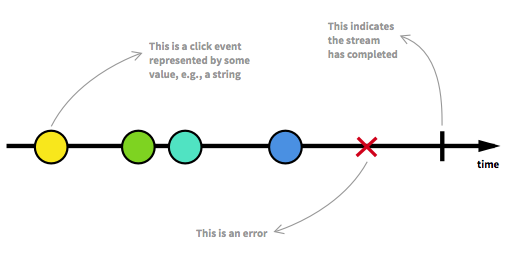
\includegraphics[width=10cm]{sygnalRx}
\caption{Schemat emitowanych danych w sygnale \cite{introToRx}}
\label{sygnalRx}
\end{figure}

Jak widać na obrazku \ref{sygnalRx}, sygnał jest ciągiem poszeregowanych zdarzeń w czasie. Przechwytywanie powyższych zdarzeń odbywa się asynchronicznie a każdy z wymienionych stanów sygnału musi być obsłużony przez zdefiniowane w tym celu funkcje. \\
\subparagraph{Obiekty Subject -}stanowią w programowaniu reaktywnym swego rodzaju most, w większości implementacji podejścia reaktywnego, ponieważ zachowują się jednocześnie jak obiekty obserwowane i obserwujące. Jako obserwatorzy, mogą zasubskrybować się do jednego lub więcej obserwowanych obiektów. Jako obserwowani mogą emitować i reemitować zdarzenia do obiektów obserwujących.\\
Rozróżnia się cztery rodzaje obiektów Subject zaprojektowanych pod konkretne przypadki.  
\subparagraph{AsyncSubject -}emituje ostatnią (i tylko ostatnią) wartość wyemitowaną przez źródołwy sygnał i tylko, gdy źródłowy sygnał zakończy się poprawnie. Jeśli źródłowy obiekt obserwowany zakończy się nie emitując żadnych wartości, obiekt AsyncSubject również zakończy się nie emitując żadnych wartości.
\begin{figure}[ht!]
	\centering
	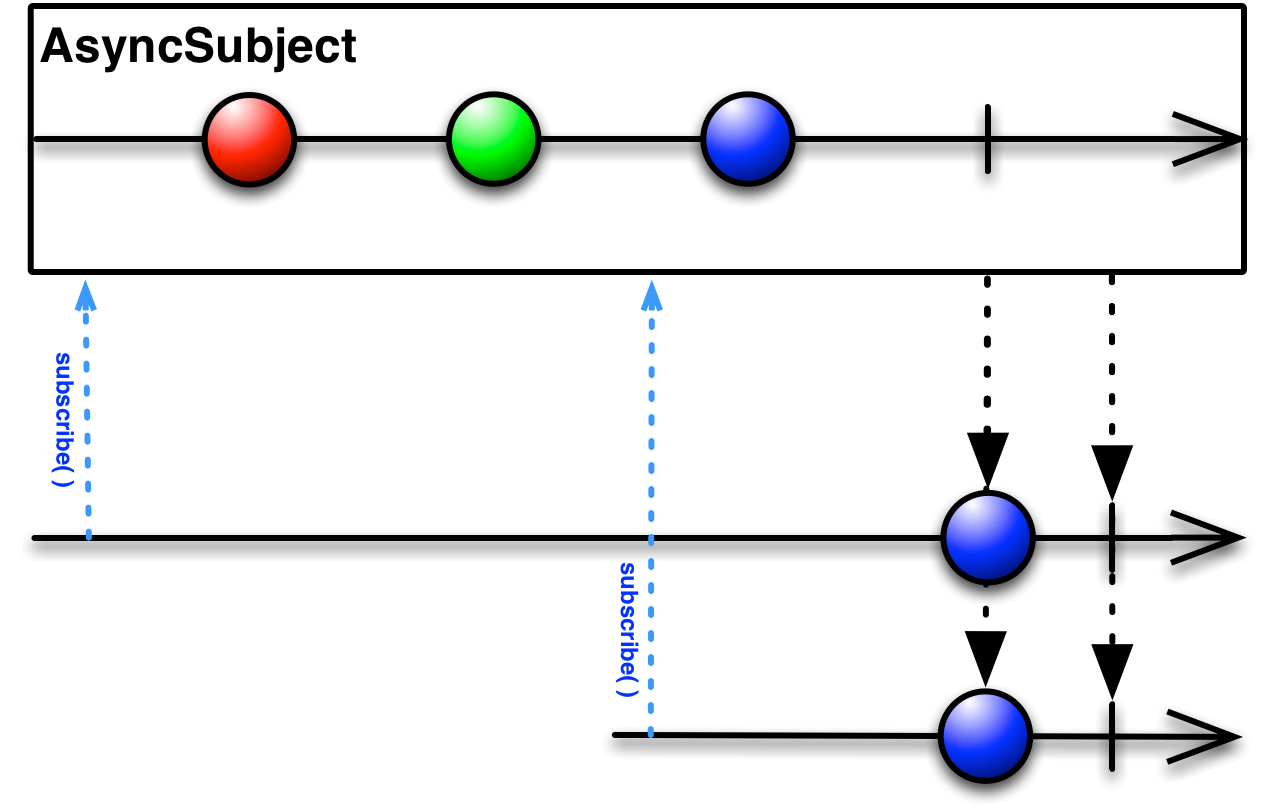
\includegraphics[width=10cm]{asyncSubject}
	\caption{Schemat poprawnie zakończonego działania obiektu AsyncSubject \cite{subjects}}
	\label{asyncSubject}
\end{figure}
\\
Rysunek \ref{asyncSubject} przedstawia sposób działanie obiektu AsyncSubject. 
Jeśli zaś źródłowy sygnał zakończy się błędem, obiekt AsyncSubject nie wyemituje żadnych wartości lecz informacje o błędzie od sygnału źródłowego.
\begin{figure}[ht!]
	\centering
	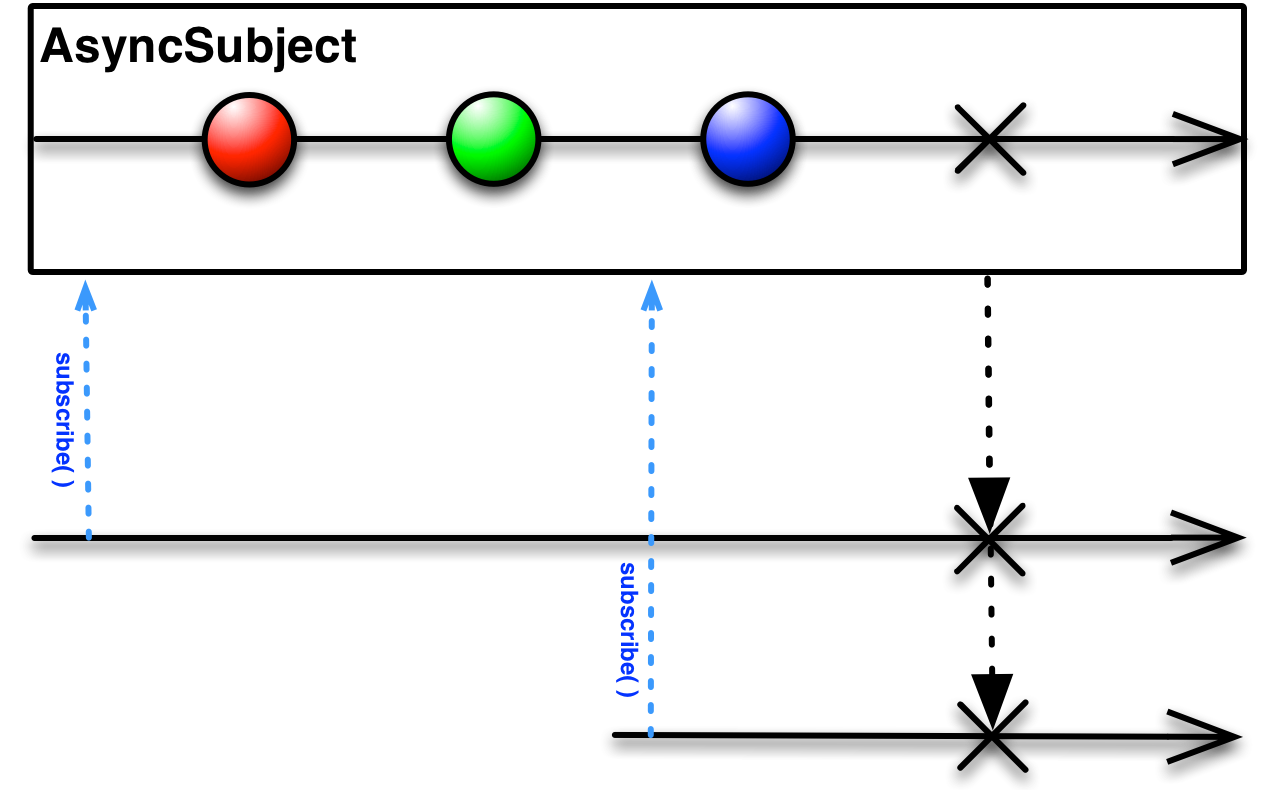
\includegraphics[width=10cm]{asyncSubjectFailed}
	\caption{Schemat działania obiektu AsyncSubject w przypadku błędu\cite{subjects}}
	\label{asyncSubjectFailed}
\end{figure}\\
Rysunek \ref{asyncSubjectFailed} przedstawia sposób działanie obiektu AsyncSubject w przypadku błędu. 
\subparagraph{BehaviorSubject -}gdy obserwator zasubskrybuje się do obiektu BehaviorSubject, rozpoczyna on emitowanie zdarzeń rozpoczynając od ostatniego uprzednio wyemitowanego przez źródłowy sygnał a następnie kontynuuje emitowanie kolejnych zdarzeń sygnału źródłowego.
\begin{figure}[ht!]
	\centering
	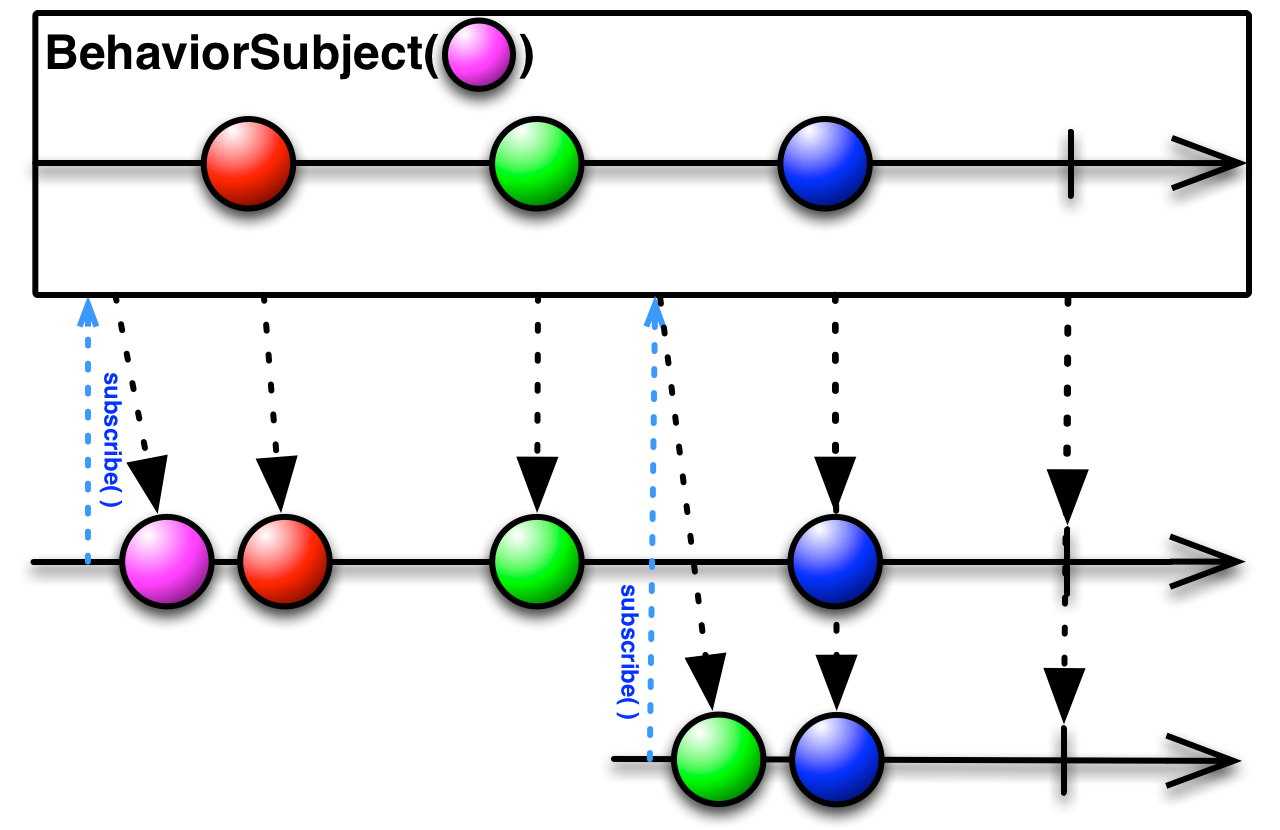
\includegraphics[width=10cm]{behaviorSubject}
	\caption{Schemat działania obiektu BehaviorSubject\cite{subjects}}
	\label{behaviorSubject}
\end{figure}
\\
\\
\\
Rysunek \ref{behaviorSubject} przedstawia sposób działanie obiektu BehaviorSubject. 
Jeśli zaś źródłowy sygnał zakończy się błędem, obiekt BehaviorSubject nie wyemituje żadnych danych do kolejnych obserwatorów, lecz prześle informacje o błędzie z obiektu źródłowego.
\begin{figure}[ht!]
	\centering
	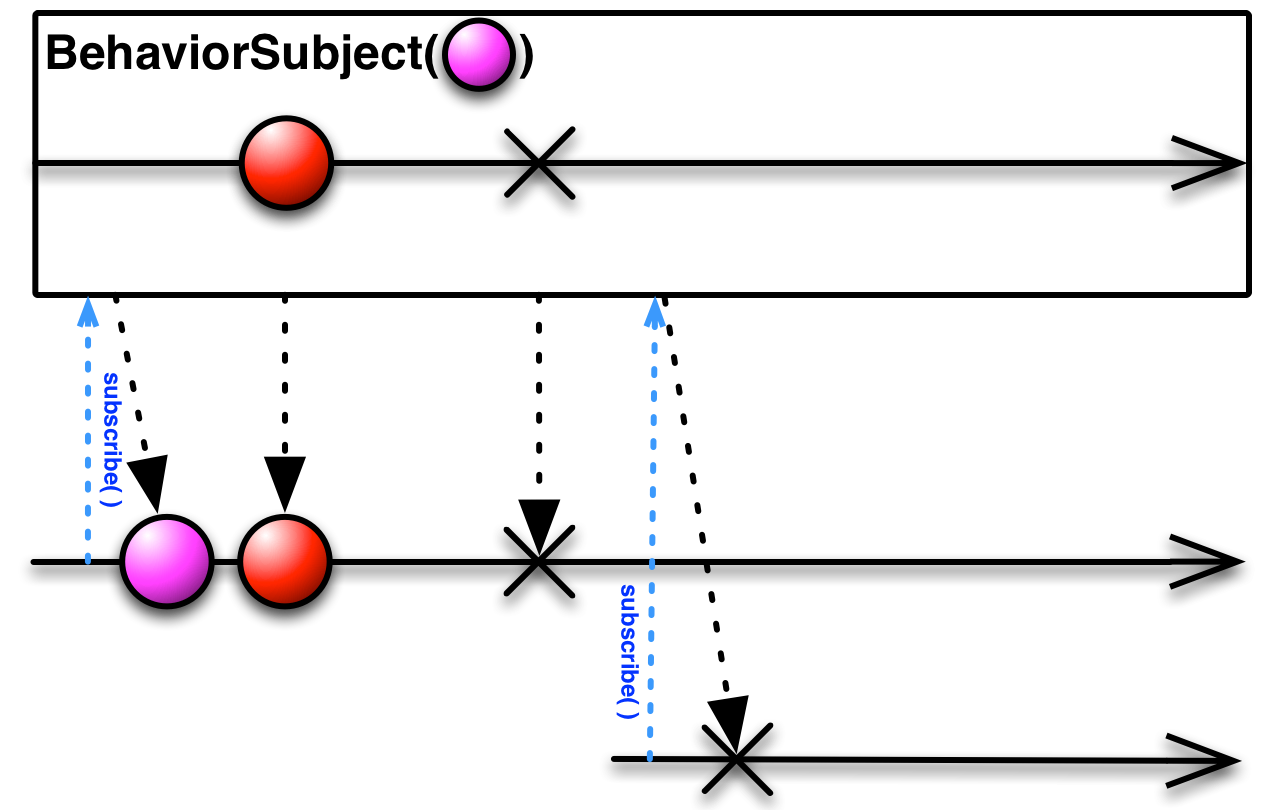
\includegraphics[width=10cm]{behaviorSubjectFailed}
	\caption{Schemat działania obiektu BehaviorSubject w przypadku błędu\cite{subjects}}
	\label{behaviorSubjectFailed}
\end{figure}
Rysunek \ref{behaviorSubjectFailed} przedstawia sposób działania obiektu BehaviorSubject w przypadku błędu.
\subparagraph{PublishSubject -}emituje do obserwatora wszystkie dane wyemitowane od momentu subskrypcji. Obiekt PublishSubject może rozpocząć emitowanie danych bezpośrednio po utworzeniu. Istnieje zatem ryzyko, że jedno lub więcej wyemitowanych zdarzeń może zostać zgubiona od czasu powstania obiektu Subject i obserwatora subskrybującego się do niego. Aby temu zapobiec, można przekształcić sygnał w "zimny" przez manualne użycie funkcji Create i upewnienie się, że zdarzenia nie są emitowane dopóki wszyscy obserwatorzy sie nie zasubskrybują. 
\begin{figure}[ht!]
	\centering
	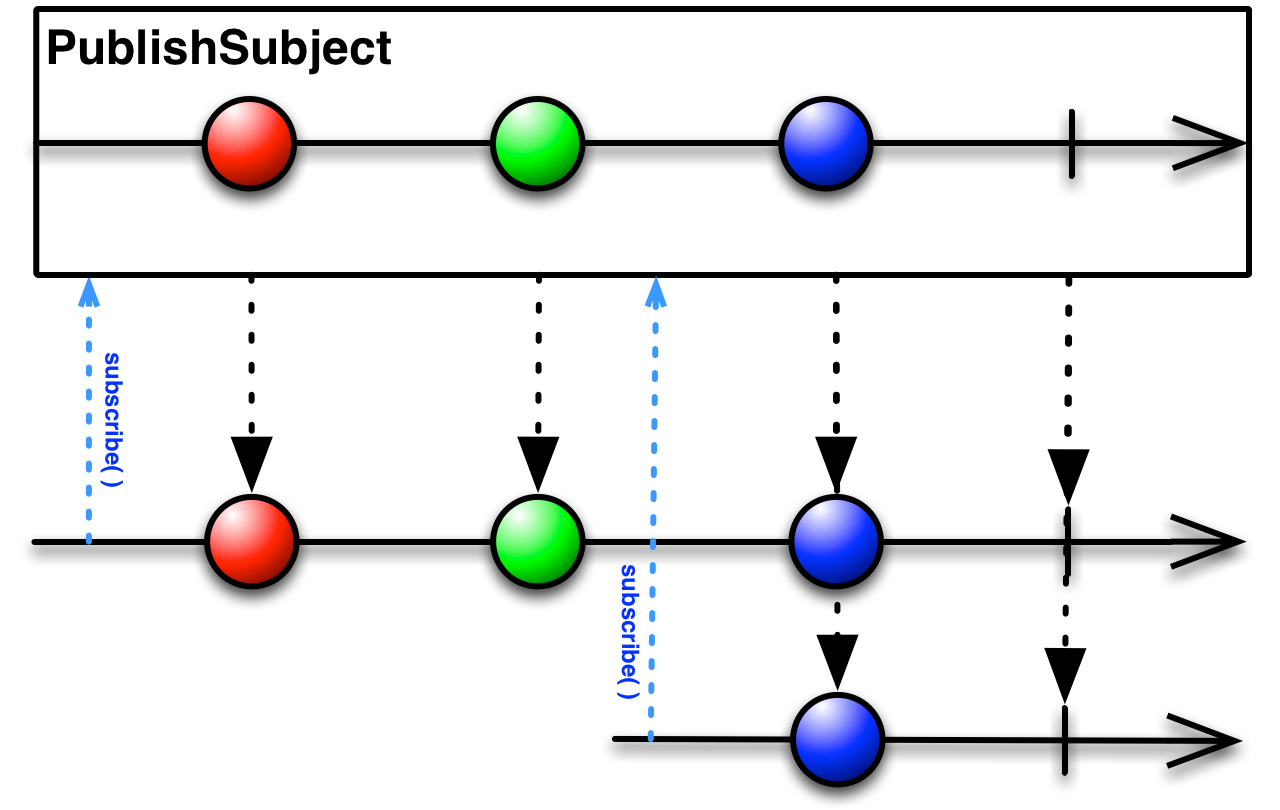
\includegraphics[width=10cm]{publishSubject}
	\caption{Schemat działania obiektu PublishSubject\cite{subjects}}
	\label{publishSubject}
\end{figure}
\\
\\
Rysunek \ref{publishSubject} przedstawia sposób działanie obiektu PublishSubject. 
Jeśli zaś źródłowy sygnał zakończy się błędem, obiekt PublishSubject nie wyemituje danych, lecz prześle informacje o błędzie z obiektu źródłowego.
\begin{figure}[ht!]
	\centering
	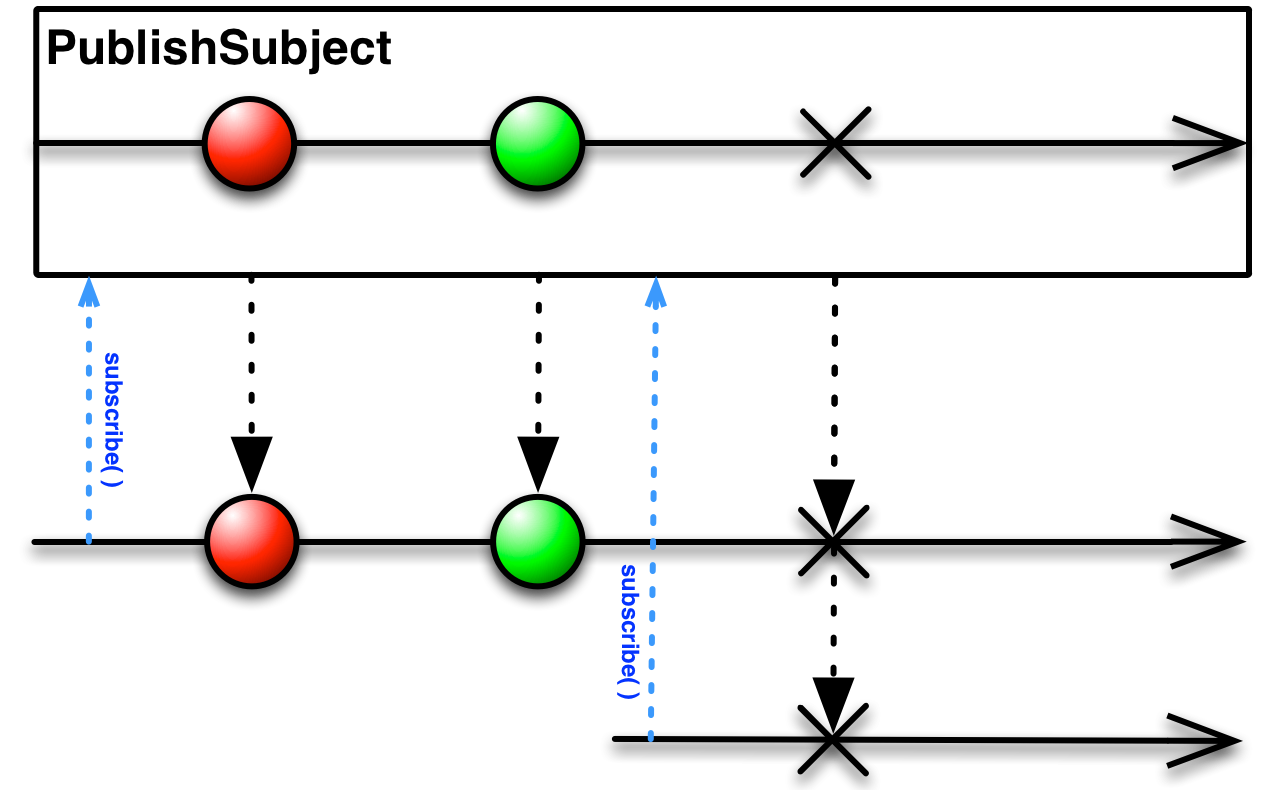
\includegraphics[width=10cm]{publishSubjectFailed}
	\caption{Schemat działania obiektu PublishSubject w przypadku błędu\cite{subjects}}
	\label{publishSubjectFailed}
\end{figure}
Rysunek \ref{publishSubject} przedstawia sposób działanie obiektu PublishSubject w przypadku błędu.
\subparagraph{ReplaySubject -}emituje do obserwatorów wszystkie zdarzenia wyemitowane przez sygnał źródłowy, bez względu na moment subskrybcji. 
\begin{figure}[ht!]
	\centering
	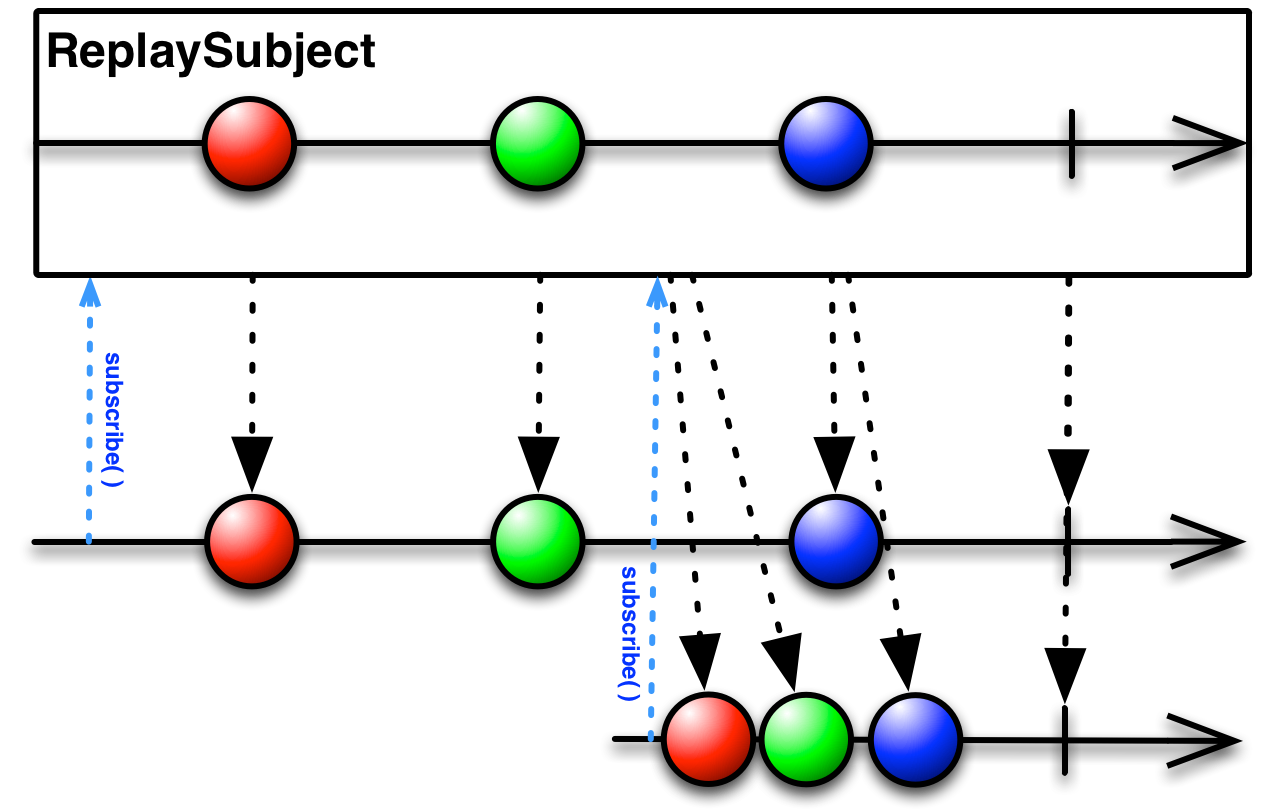
\includegraphics[width=10cm]{replaySubject}
	\caption{Schemat działania obiektu ReplaySubject\cite{subjects}}
	\label{replaySubject}
\end{figure}\\
Rysunek \ref{replaySubject} przedstawia sposób działanie obiektu ReplaySubject.
Możliwa jest implementacja obiektu ReplaySubject, której działanie będzie polegało na odrzuceniu starych zdarzeń, czyli obostrzonych rozmiarem bufora bądź upływem zadanej ilości czasu.\\
Obiekt ReplaySubject używany jako obserwator, dba o to by jego metoda onNext (lub inne metody on) nie były wywoływane z różnych wątków. Może to doprowadzić do powielania już raz wyemitowanych zdarzeń i niejednoznaczności, co stoi w sprzeczności z wytycznymi projektowymi paradgymatu reaktywnego.\cite{rxDesignGuideline} 
\subsection{Operatory reaktywne}
\paragraph{}Znaczna część operatorów reaktywnych została zaczerpnięta z podejścia funkcyjnego. Mają na celu umożliwienie tworzenia sygnałów, przekształcania w inne, filtrowania, łączenia, obsługi błędów, itp.\\
Większość operatorów programowania reaktywnego działa na obiekcie typu Observable a wynikiem działania jest obiekt typu Observable. Dlatego stosowane jest podejście łączenia operacji w całe łańcuchy działań na sygnałach. Należy tu jednak podkreślić, że kolejne operatory łańcucha nie działają na oryginalnym obiekcie Observable niezależnie. Operują one kolejno na wynikach poprzednich działań w łańcuchu czyli na kolejnych obiektach Observable. \\
W dalszej części tego paragrafu zostaną scharakteryzowane najczęściej stosowane operatory reaktywne.
\paragraph{Operatory tworzenia sygnałów}
\subparagraph{Create -}tworzy od podstaw obiekt Observable. Do operatora podawana jest funkcja przyjmująca w argumencie obiekt obserwującego. Tworzy się za jej pomocą obiekt obserwowany, przez zdefniowanie działań funkcji onNext, onError i onCompleted. 
\begin{figure}[ht!]
	\centering
	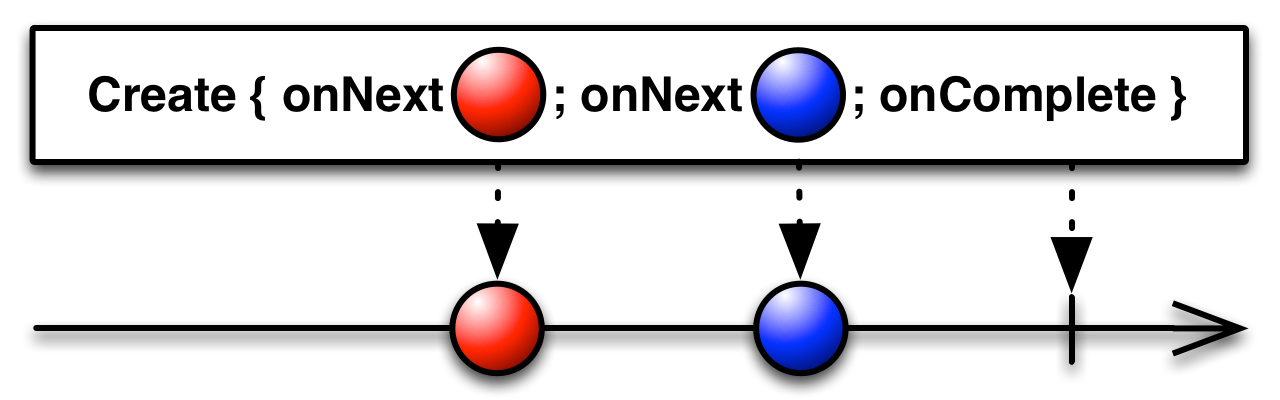
\includegraphics[width=6cm]{create}
	\caption{Schemat działania operatora Create\cite{operators}}
	\label{create}
\end{figure}\\
Rysunek \ref{create} przedstawia działanie operatora Create.
\subparagraph{Defer -}tworzy obiekt Observable, ale dopiero gdy obserwator się do niego zasubskrybuje. Działanie to jest powielane dla każdego subskrybenta, dlatego, pomimo iż wszyscy nasłuchują z tego samego sygnału, otrzymują indywidualne sekwencje zdarzeń. 
\begin{figure}[ht!]
	\centering
	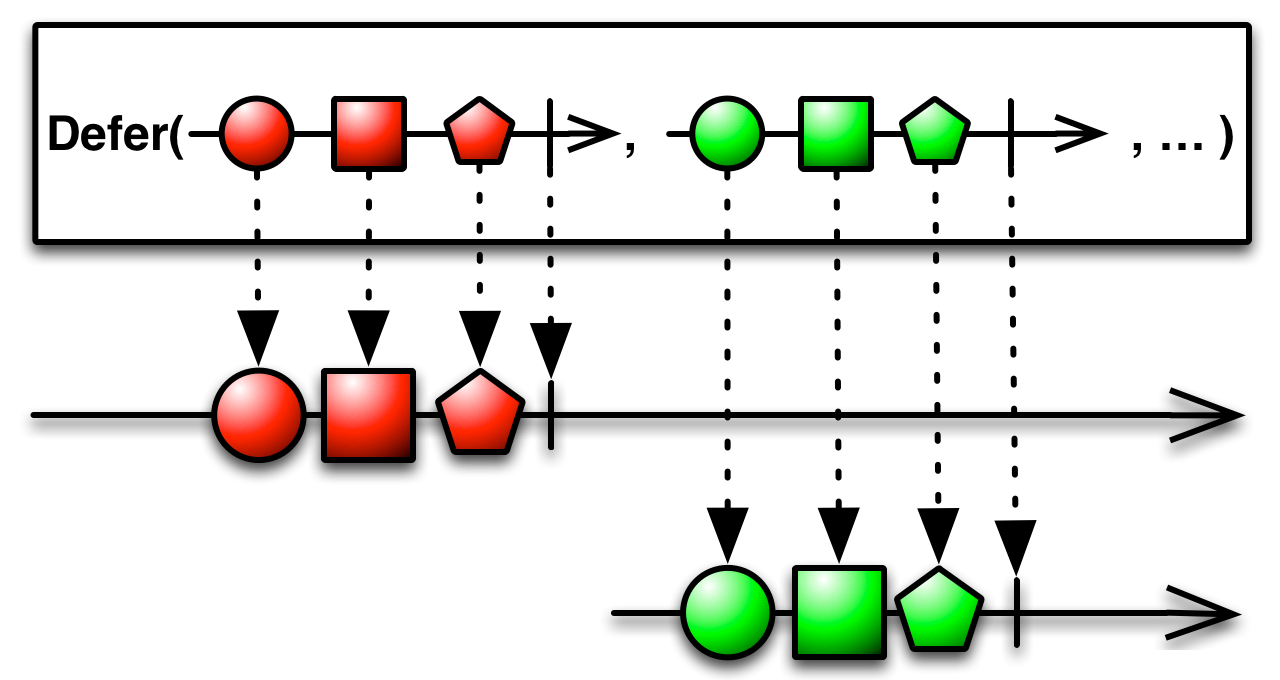
\includegraphics[width=6cm]{defer}
	\caption{Schemat działania operatora Defer\cite{operators}}
	\label{defer}
\end{figure}\\\\\\\\\\\\
Rysunek \ref{defer} przedstawia działanie operatora Defer.
\paragraph{Operatory przekształcania sygnałów}
\subparagraph{Buffer -}cyklicznie zbiera generowane przez obiekt Observable zdarzenia i emituje w postaci pakietów zdarzeń. W przypadku napotkania błędu przez obiekt obserwowany, operator Buffer wyemituje zdarzenie informujące o błędzie bez wytworzenia pakietu danych.
\begin{figure}[ht!]
	\centering
	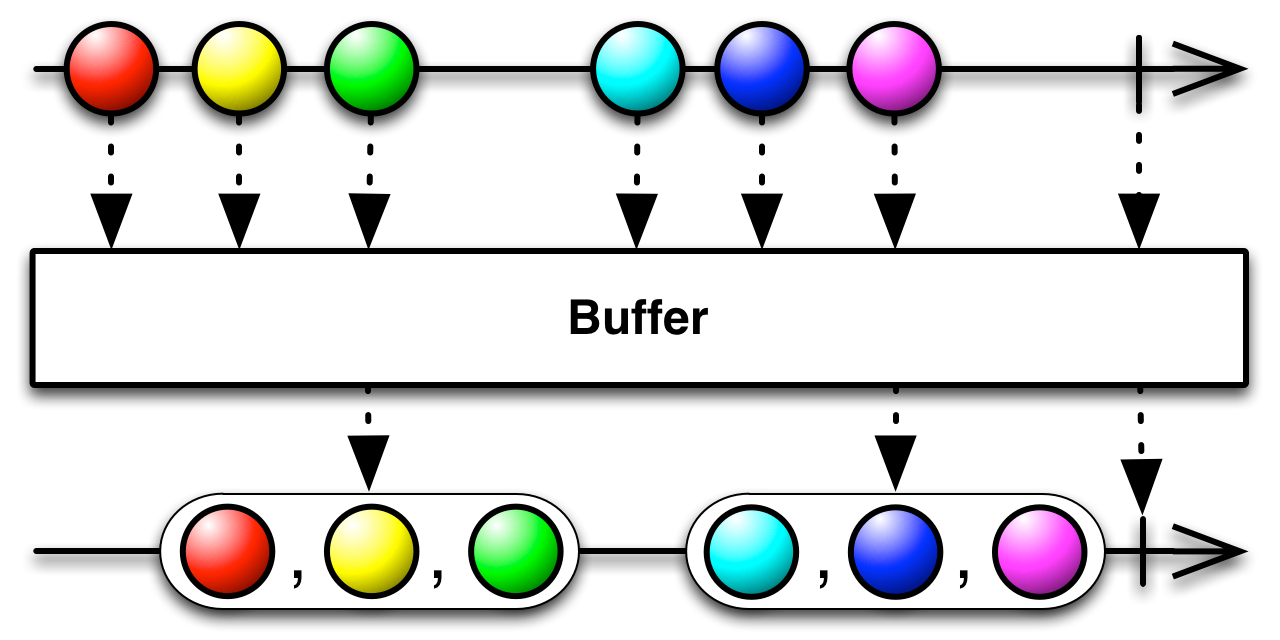
\includegraphics[width=6cm]{buffer}
	\caption{Schemat działania operatora Buffer\cite{buffer}}
	\label{buffer}
\end{figure}\\
Rysunek \ref{buffer} przedstawia działanie operatora Buffer.
\subparagraph{FlatMap -}przekształca obiekt Observable przez zastosowanie funkcji zdefiniowanej dla każdego wyemitowanego zdarzenia przez źródłowy obiekt obserwowany, gdzie funkcja ta zwraca obiekt Observble emitujący własne zdarzenia. Nastepnie operator flatMap scala emisje wynikowych obiektów Observable w jedną sekwencję danych.
\begin{figure}[ht!]
	\centering
	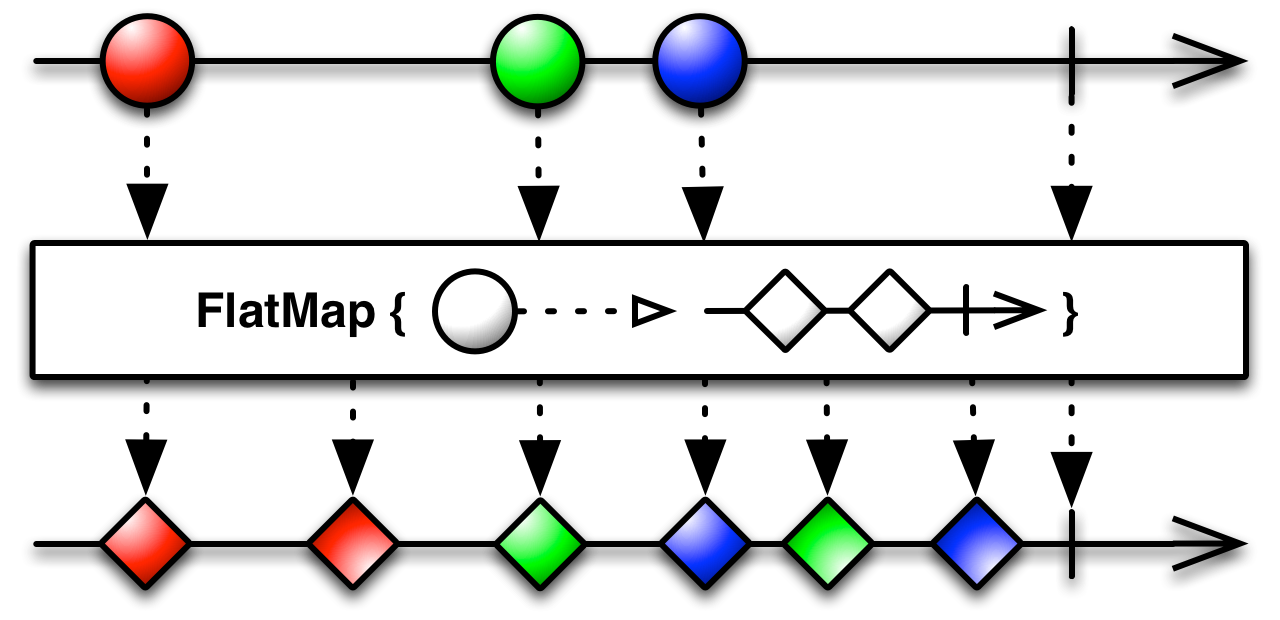
\includegraphics[width=6cm]{flatmap}
	\caption{Schemat działania operatora FlatMap\cite{operators}}
	\label{flatmap}
\end{figure}\\\\\\\\\\\\\\
Rysunek \ref{flatmap} przedstawia działanie operatora FlatMap.
\subparagraph{Map -}stosuje zdefiniowaną funkcję do każdego wyemitowanego przez źródłowy obiekt Observable zdarzenia a następnie zwraca obiekt Observable emitujący przekształcone tą funkcją zdarzenia.
\begin{figure}[ht!]
	\centering
	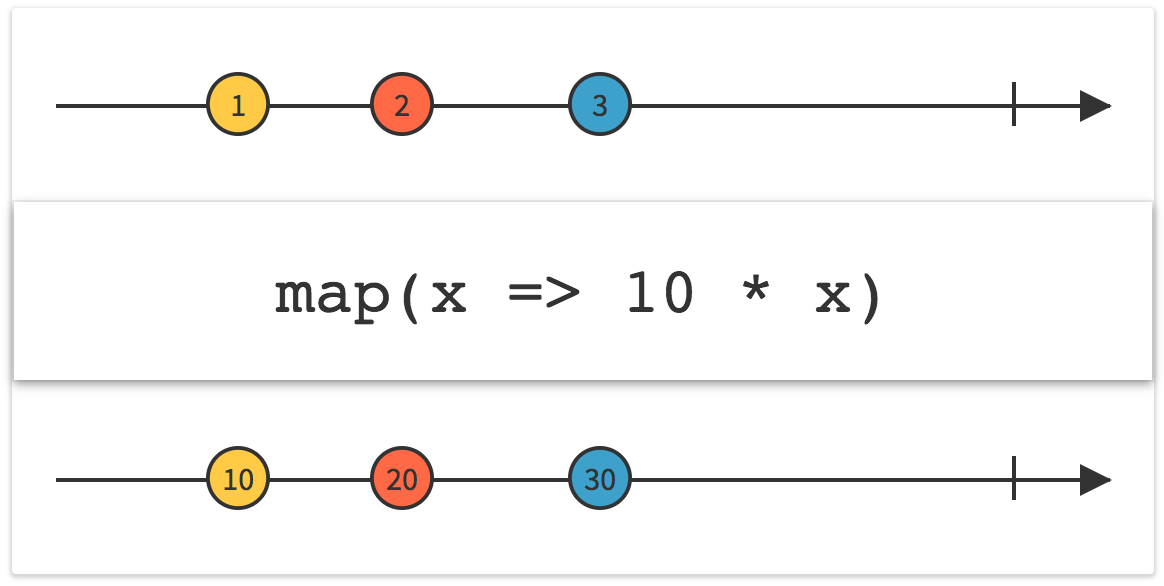
\includegraphics[width=6cm]{map}
	\caption{Schemat działania operatora Map\cite{marbles}}
	\label{map}
\end{figure}\\
Rysunek \ref{map} przedstawia działanie operatora Map.
\subparagraph{Scan -}stosuje zdefiniowaną funkcję do pierwszego wyemitowanego przez źródło zdarzenia a następnie emituje to przekształcone zdarzenie jako swoje pierwsze. Wynik tego zdarzenia podawany jest spowrotem to funkcji wraz z kolejnym zdarzeniem z obiektu źródłowego i emitowany.
\begin{figure}[ht!]
	\centering
	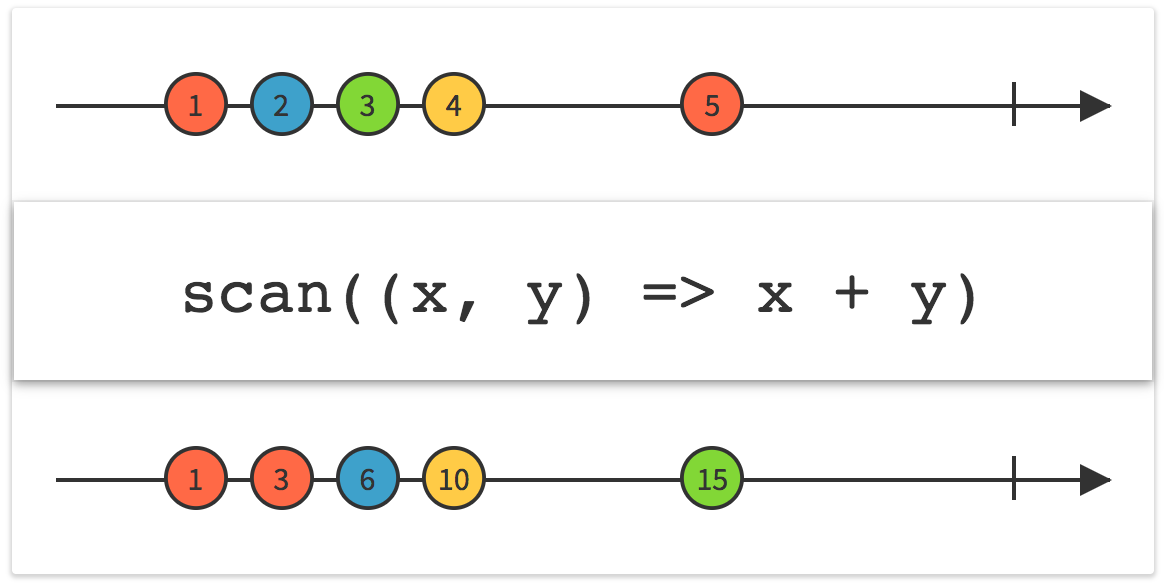
\includegraphics[width=6cm]{scan}
	\caption{Schemat działania operatora Scan\cite{marbles}}
	\label{scan}
\end{figure}
Rysunek \ref{scan} przedstawia działanie operatora Scan.
\pagebreak
\paragraph{Operatory filtrowania sygnałów}
\subparagraph{Debounce -}emituje zdarzenie z obiektu Observable tylko po upływie zadanego interwału czasowego bez emisji zdarzenia.
\begin{figure}[ht!]
	\centering
	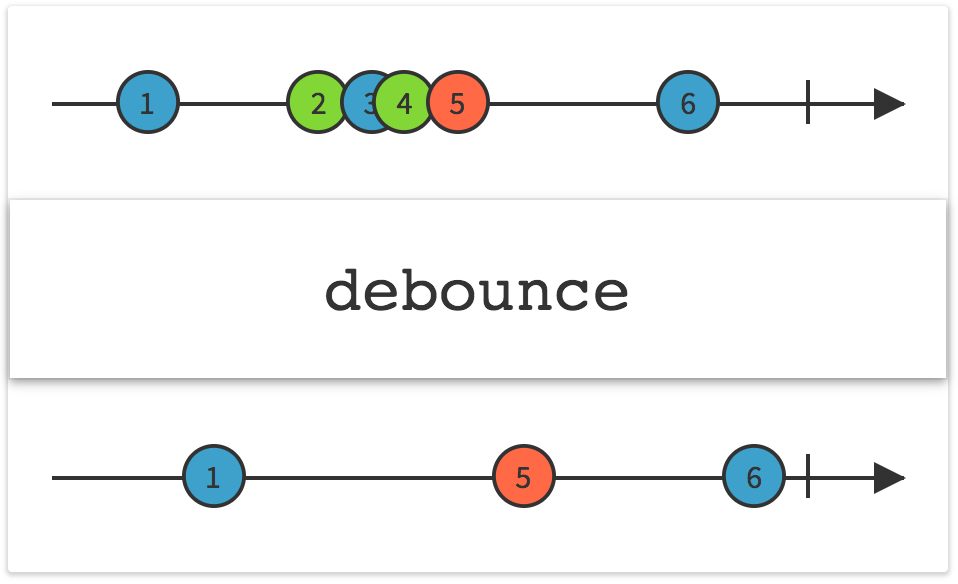
\includegraphics[width=6cm]{debounce}
	\caption{Schemat działania operatora Debounce\cite{marbles}}
	\label{debounce}
\end{figure}\\
Rysunek \ref{debounce} przedstawia działanie operatora Debounce.
\subparagraph{Distinct -}ignoruje wartości już raz wyemitowane.
\begin{figure}[ht!]
	\centering
	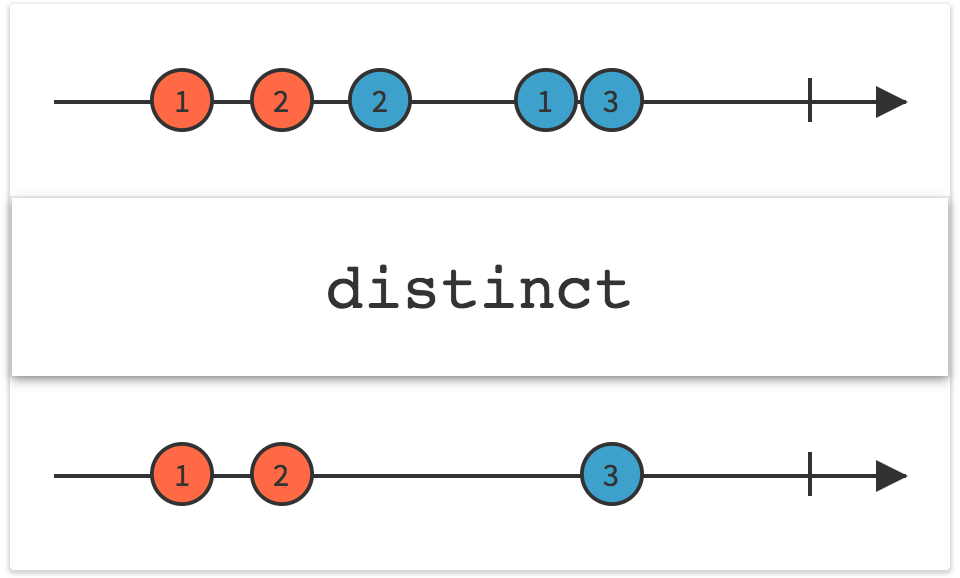
\includegraphics[width=6cm]{distinct}
	\caption{Schemat działania operatora Distinct\cite{marbles}}
	\label{distinct}
\end{figure}\\
Rysunek \ref{distinct} przedstawia działanie operatora Distinct.
\subparagraph{Filter -}odfiltrowuje zdarzenia emitowane przez obiekt Observable, spełniające wymagania zadanej funkcji lub predykatu.
\begin{figure}[ht!]
	\centering
	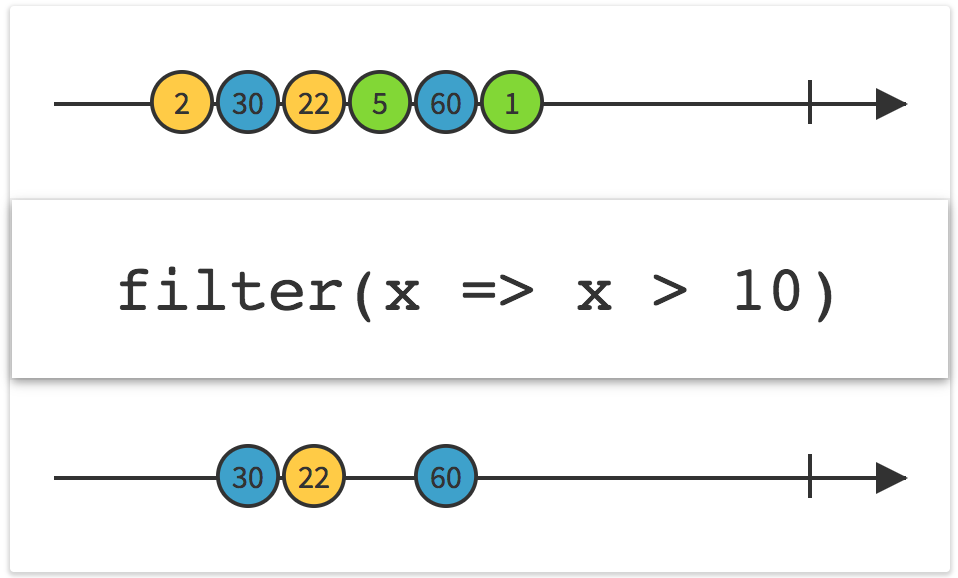
\includegraphics[width=6cm]{filter}
	\caption{Schemat działania operatora Filter\cite{marbles}}
	\label{filter}
\end{figure}
\\\\\\\\\\\\\\\\\\
Rysunek \ref{filter} przedstawia działanie operatora Filter.
\subparagraph{Skip -}ignoruje n wygenerowanych przez obiekt Observable zdarzeń, gdzie n jest liczbą naturalną, będącą parametrem.
\begin{figure}[ht!]
	\centering
	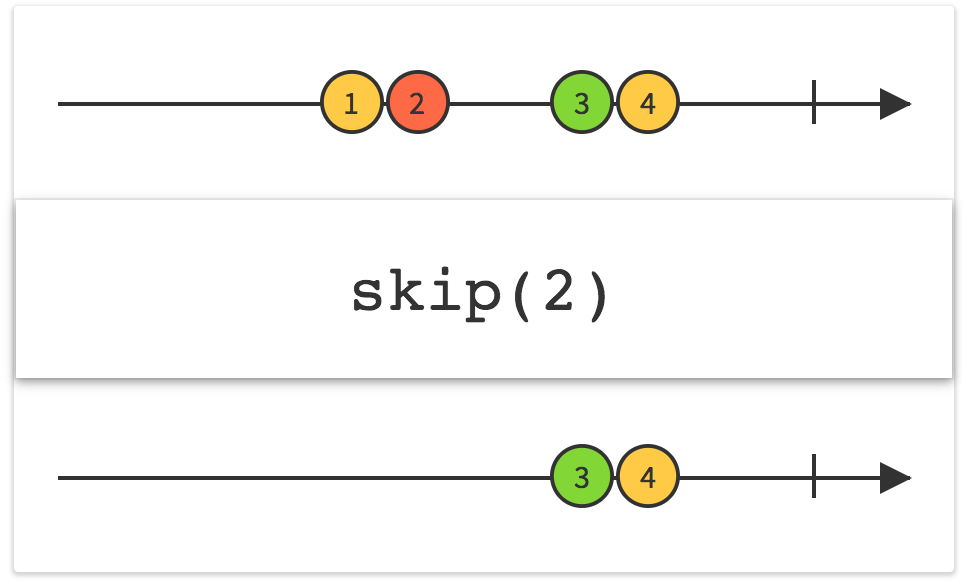
\includegraphics[width=6cm]{skip}
	\caption{Schemat działania operatora Skip\cite{marbles}}
	\label{skip}
\end{figure}
Rysunek \ref{skip} przedstawia działanie operatora Skip.
\subparagraph{Take -}emituje pierwsze n wydarzeń wygenerowanych przez obiekt Observable, gdzie n jest liczbą naturalną, będącą parametrem.
\begin{figure}[ht!]
	\centering
	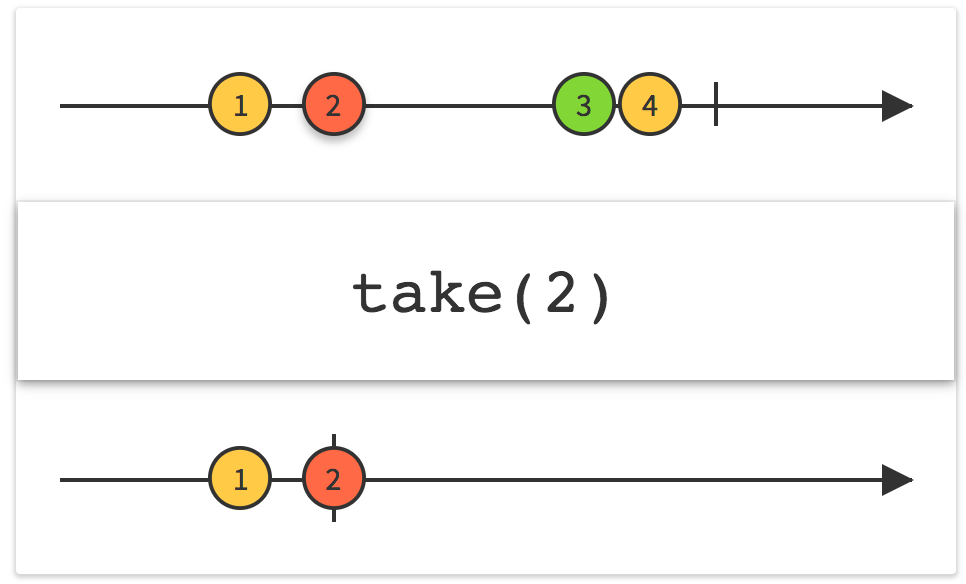
\includegraphics[width=6cm]{take}
	\caption{Schemat działania operatora Take\cite{marbles}}
	\label{take}
\end{figure}
Rysunek \ref{take} przedstawia działanie operatora Take.
\pagebreak
\paragraph{Operatory łączenia}
\subparagraph{CombineLatest -}łączy ostatnie wyemitowane zdarzenia zadaną funkcją (strategią) z dwóch lub więcej źródeł i emituje nowe zdarzenie będące wynikiem powyższych. 
\begin{figure}[ht!]
	\centering
	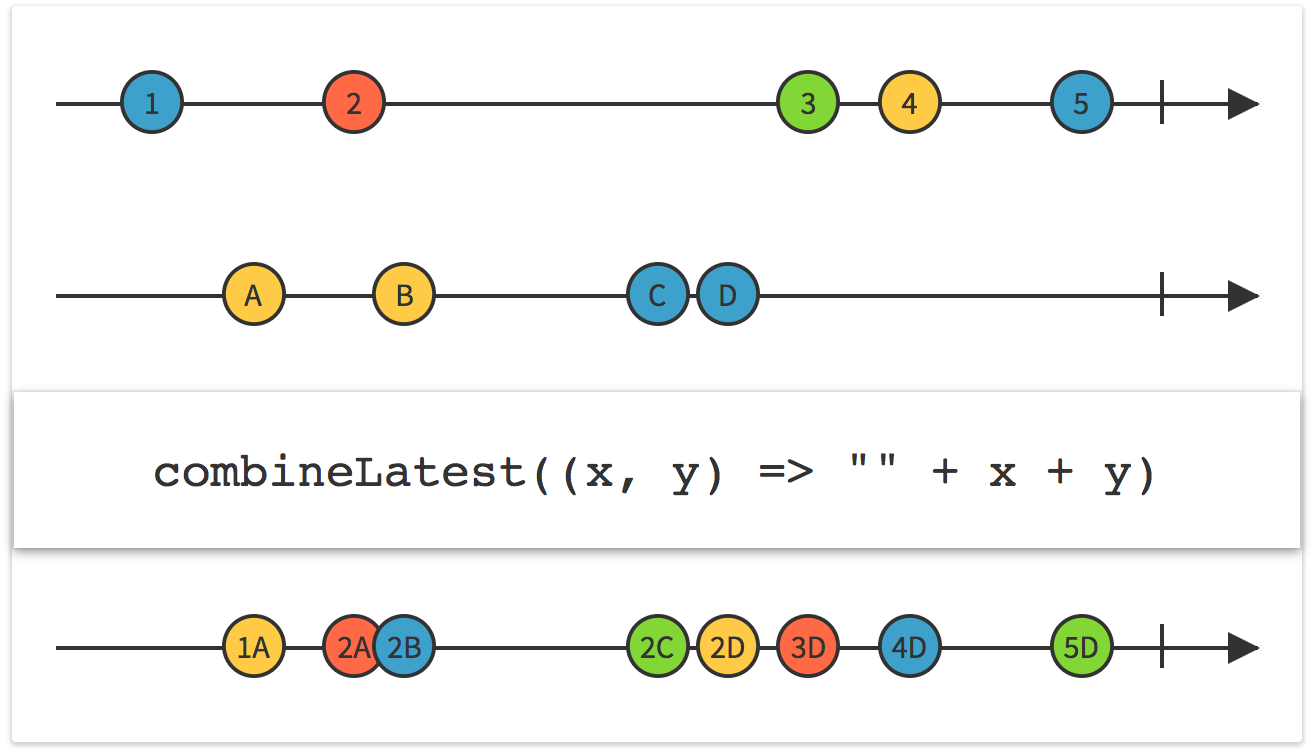
\includegraphics[width=8cm]{combinelatest}
	\caption{Schemat działania operatora CombineLatest\cite{marbles}}
	\label{combinelatest}
\end{figure}\\
Rysunek \ref{combineLatest} przedstawia działanie operatora CombineLatest.
\subparagraph{Merge -}łączy zdarzenia emitowane z wielu sygnałów w jeden ciągły sygnał zdarzeń
\begin{figure}[ht!]
	\centering
	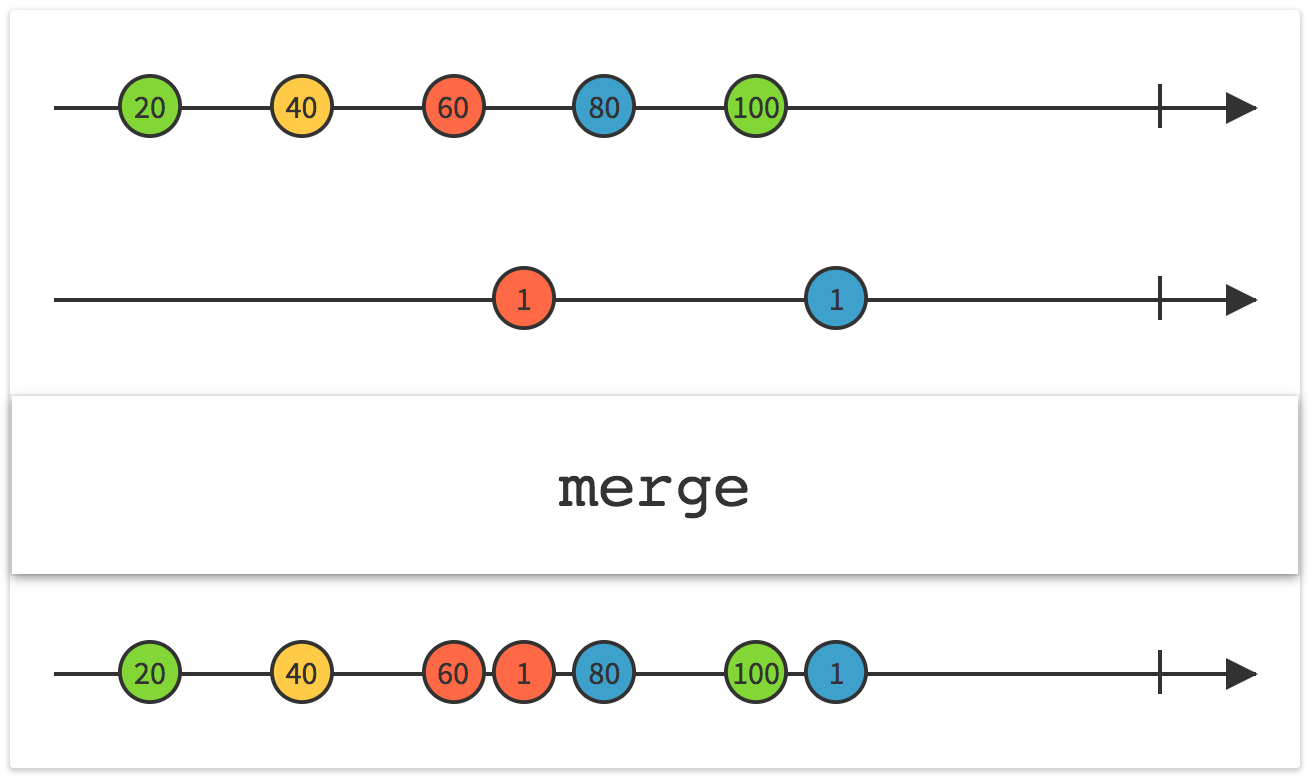
\includegraphics[width=8cm]{merge}
	\caption{Schemat działania operatora Merge\cite{marbles}}
	\label{merge}
\end{figure}\\
Rysunek \ref{merge} przedstawia działanie operatora Merge.
\subparagraph{Zip -}łączy zdarzenia emitowane z dwóch lub więcej sygnałów w pojedyncze zdarzenia reprezentowane krotką. 
\begin{figure}[ht!]
	\centering
	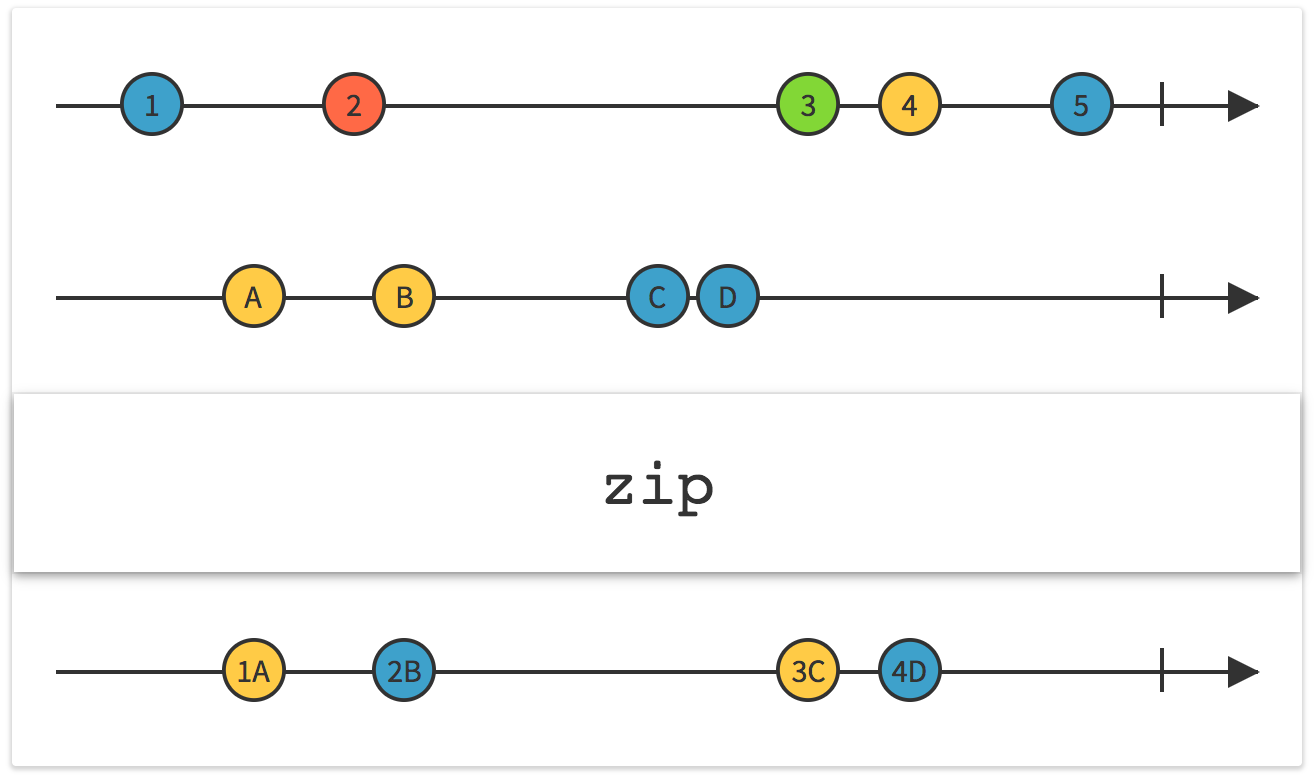
\includegraphics[width=8cm]{zip}
	\caption{Schemat działania operatora Zip\cite{zip}}
	\label{zip}
\end{figure}\\
Rysunek \ref{zip} przedstawia działanie operatora Zip.
\paragraph{Operatory obsługi błędów}
\subparagraph{Catch -}operator ten przechwytuje zdarzenie onError od obiektu Observable i zamiast propagować błąd do obserwujących, podmienia zdarzenie na inne dane lub inny zestaw danych, co pozwala zakończyć się wynikowemu obiektowi Observable w normalny sposób (onCompleted) lub nie zakończyć się w cale.
\begin{figure}[ht!]
	\centering
	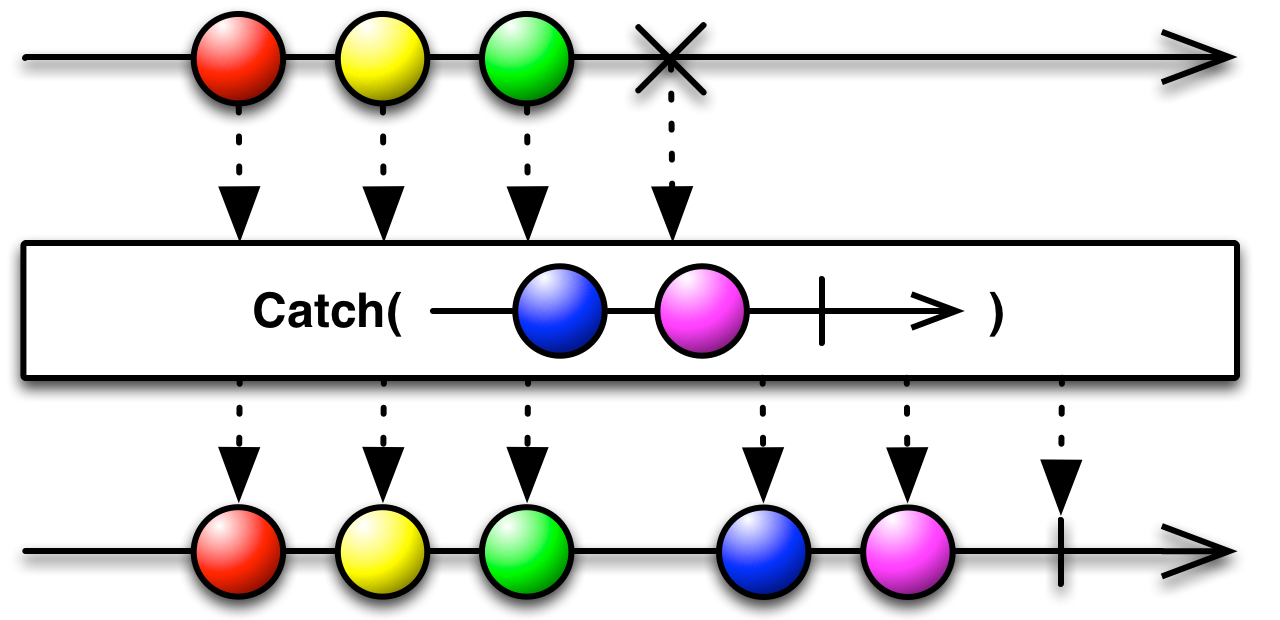
\includegraphics[width=8cm]{catch}
	\caption{Schemat działania operatora Catch\cite{operators}}
	\label{catch}
\end{figure}\\
Rysunek \ref{catch} przedstawia działanie operatora Catch.
\subparagraph{Retry -}w przypadku odebrania od obiektu Observable zdarzenia onError, operator Retry nie propaguje błędu do obiektów obserwujących. Zamiast tego wykonywana jest resubskrybcja do źródłowego sygnału. Operator Retry zawsze przekazuje zdarzenie onNext do swoich obserwatorów, nawet z ciągów kończących się błędem. Może to powodować zduplikowanie wyemitowania zdarzenia.
\begin{figure}[ht!]
	\centering
	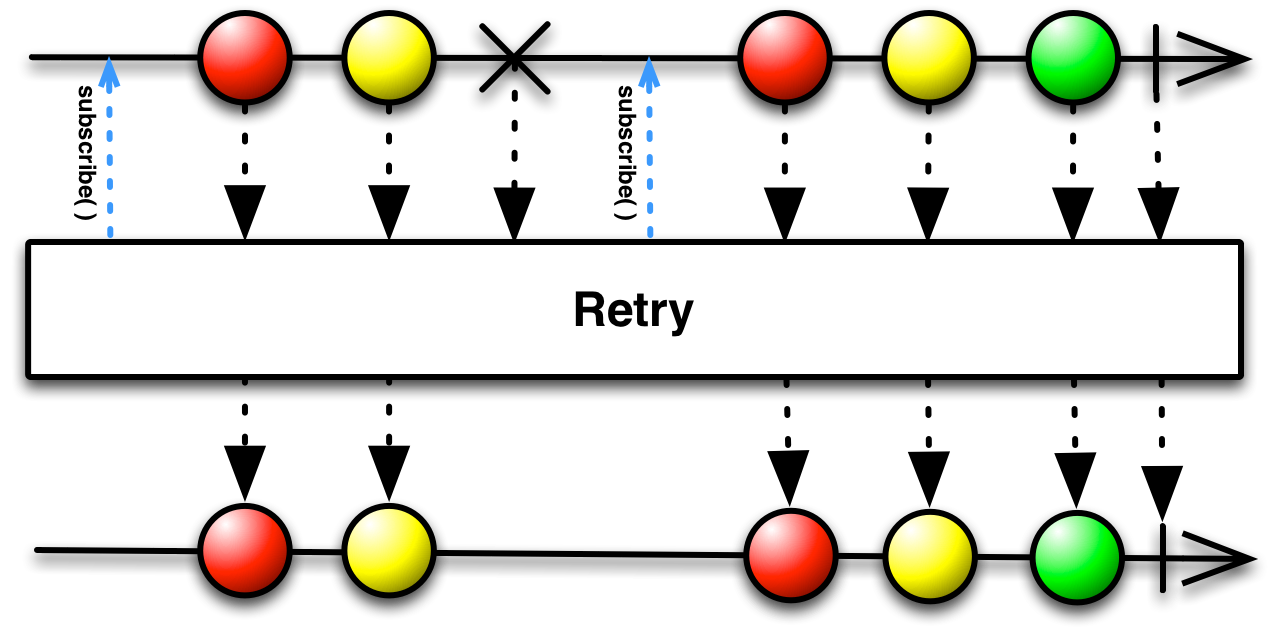
\includegraphics[width=8cm]{retry}
	\caption{Schemat działania operatora Retry\cite{operators}}
	\label{retry}
\end{figure}\\
Rysunek \ref{retry} przedstawia działanie operatora Retry.
\paragraph{Operatory działań na obiektach Observable}
\subparagraph{Materialize -}konwertuje sekwencje emitowanych z obiektu Observable zdarzeń, na sekwencję zdarzeń reprezentowanych przez wywołania metod onNext i ostatecznie onCompleted lub onError.
\begin{figure}[ht!]
	\centering
	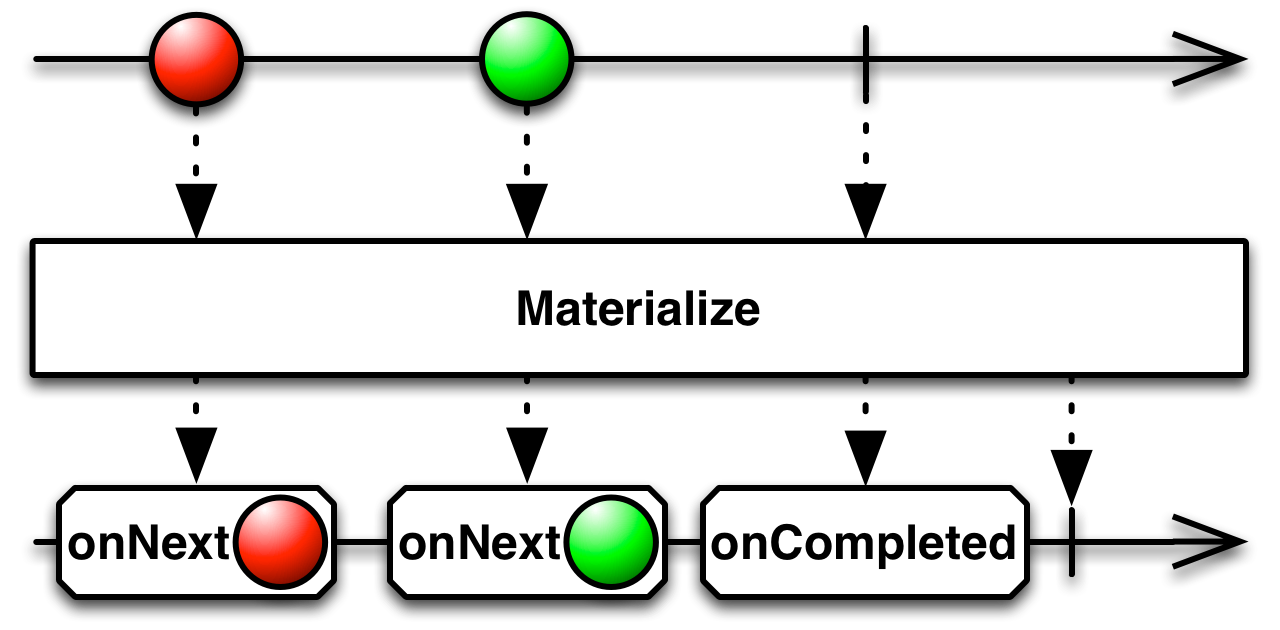
\includegraphics[width=8cm]{materialize}
	\caption{Schemat działania operatora Materialize\cite{operators}}
	\label{materialize}
\end{figure}\\
Rysunek \ref{materialize} przedstawia działanie operatora Materialize.
\subparagraph{ObserveOn -}w środowisku wielowątkowym, określa wątek, na którym obserwatorzy będą nasłuchiwali na generowane zdarzenia. 
\begin{figure}[ht!]
	\centering
	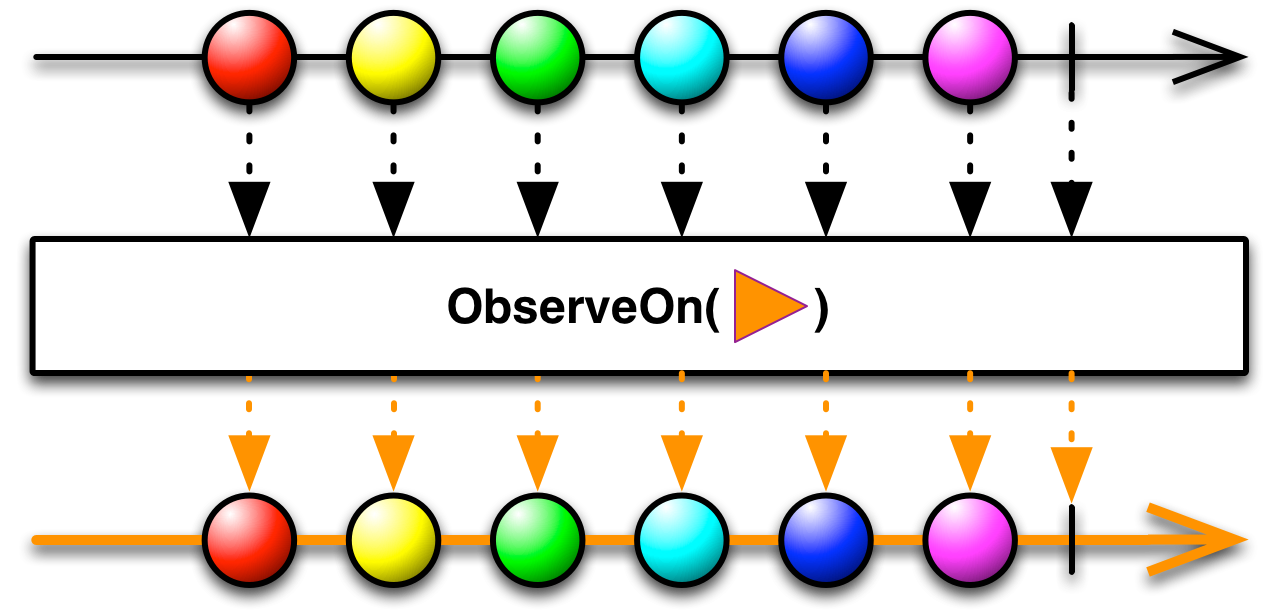
\includegraphics[width=8cm]{observeOn}
	\caption{Schemat działania operatora ObserveOn\cite{operators}}
	\label{observeOn}
\end{figure}\\
Rysunek \ref{observeOn} przedstawia działanie operatora ObserveOn.
Należy ponadto zauważyć, że ObserveOn prześle zdarzenie onError niezwłocznie, gdy je otrzyma. Oznacza to, że jeśli istnieje zasubskrybowany obserwator, wolniej przetwarzający otrzymywane zdarzenia, to możliwe jest, iż zdarzenie onError przeskoczy na miejsce przed zdarzeniami jeszcze nieprzetworzonymi przez ten obserwator. 
\begin{figure}[ht!]
	\centering
	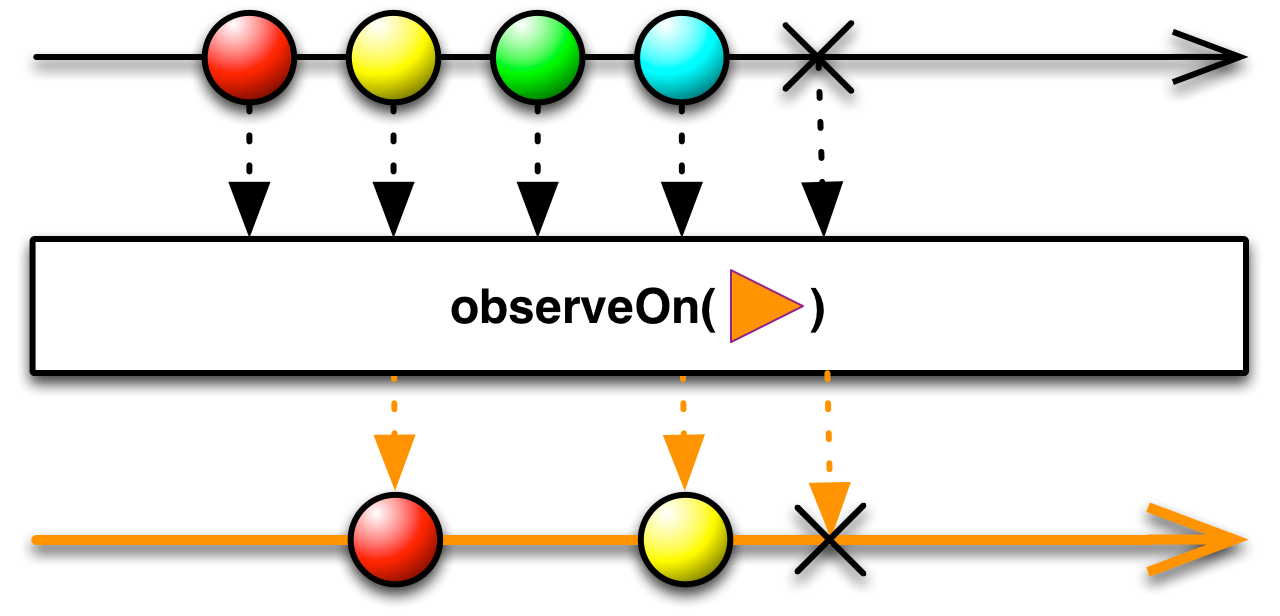
\includegraphics[width=8cm]{observeOnError}
	\caption{Schemat działania operatora ObserveOnError\cite{operators}}
	\label{observeOnError}
\end{figure}\\
Rysunek \ref{observeOnError} przedstawia działanie operatora ObserveOnError.
\subparagraph{SubscribeOn -}w środowisku wielowątkowym, określa wątek, na którym obiekt Observable będzie wykonywał pracę. Domyślnie obiekt Observable jak i ciąg zastosowanych operatorów reaktywnych, będą działały i powiadamiały obserwatorów o zdarzeniach, na tym samym wątku, na którym wywołano metodą Subscribe. Operator SubscribeOn zmienia to zachowanie, przez określenie wątku, na którym obiekt Observable będzie działał. 
\begin{figure}[ht!]
	\centering
	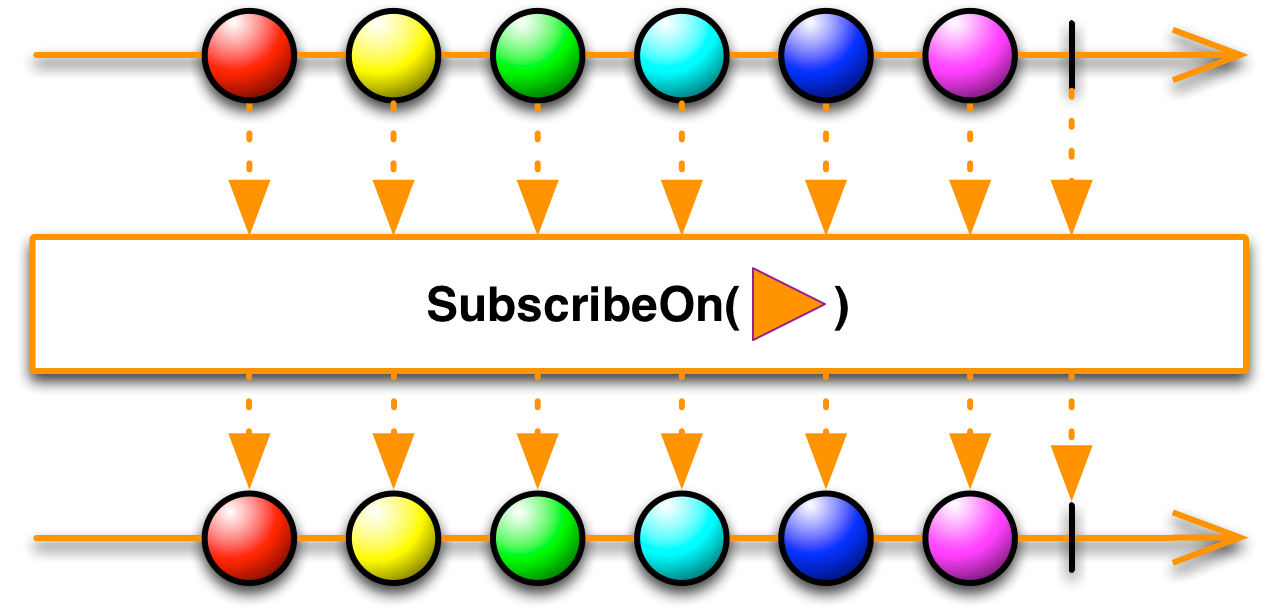
\includegraphics[width=8cm]{subscribeOn}
	\caption{Schemat działania operatora SubscribeOn\cite{operators}}
	\label{subscribeOn}
\end{figure}\\
Rysunek \ref{subscribeOn} przedstawia działanie operatora SubscribeOn.
\subparagraph{Serialize -}z racji tego, że obiekt Observable może wywoływać swoje metody asynchronicznie, na różnych wątkach, możliwe jest, że będzie próbował przesłać zdarzenie onCompleted lub onError przed jakimś innym zdarzeniem onNext lub nawet przesłać kilka różnych zdarzeń onNext z różnych wątków, współbieżnie. Takie zachowania narusza wspomniane wcześniej zalecenia odnośnie projektowania zadań w paradygmacie reaktywnym. Operator Serialize zmusza obiekt Observable do emitowania zdarzeń w sposób synchroniczny.
\begin{figure}[ht!]
	\centering
	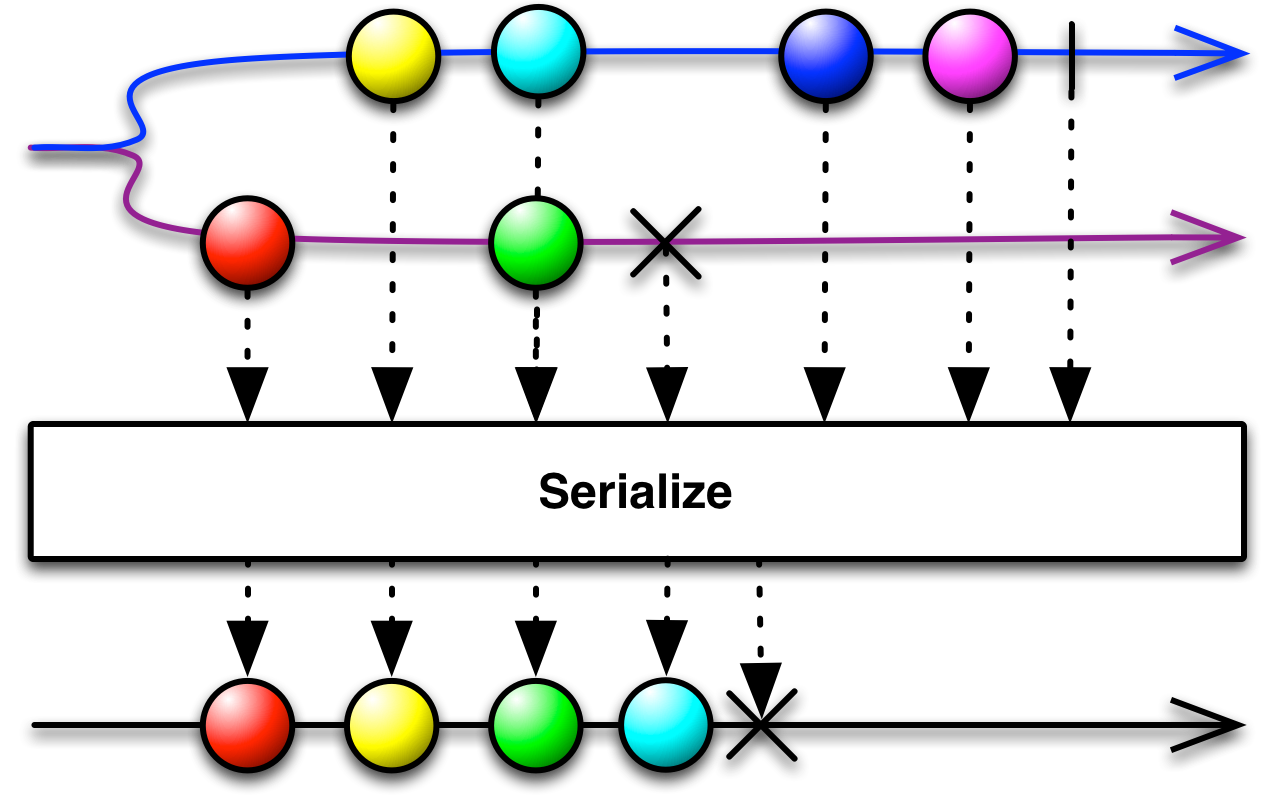
\includegraphics[width=8cm]{serialize}
	\caption{Schemat działania operatora Serialize\cite{operators}}
	\label{serialize}
\end{figure}\\
Rysunek \ref{serialize} przedstawia działanie operatora Serialize.
\subsection{Współbieżność}
\paragraph{}Podstawowym założeniem podejścia reaktywnego jest przetwarzanie danych w sposób asynchroniczny. Aby zapewnić efektywny poziom asynchroniczności wykonywanych działań, wymagany jest pewien poziom współbieżności, czyli przetwarzania danych w oparciu o współistnienie wielu wątków lub procesów.
\paragraph{Planiści (Schedulers)}
Narzędziem do zaimplementowania wielowątkowości podczas tworzenia łańcuchów sygnałów połączonych operatorami reaktywnymi, są tzw. planiści (ang. schedulers).\\
Niektóre operatory reaktywne, jako parametr przyjmują planistę, obiekt Scheduler, reprezentujący wątek, na którym ma być wykonywana praca.\\
Domyślnie, obiekt Observable i zastosowany do niego łańcuch operatorów, wykonują pracę i informują obserwatorów na tym samym wątku, na którym wywołano subskrybcję (metoda Subscribe).\\
Jak opisano wcześniej, operator SubscribeOn zmienia to zachowanie, przez określenie innego planisty (schedulera), na którym ma operować obiekt Observable. Operator ObserveOn zaś, określa planistę (scheduler), którego obiekt Observable ma użyć do wysyłania zdarzeń do swoich obserwatorów.\\
Jak pokazano na poniższej ilustracji, operator SubscribeOn określa wątek, na którym obiekt Observable rozpocznie swoje działanie, bez względu na to, w którym miejscu łańcucha operatorów zostanie on wywołany. Z drugiej zaś strony, operator ObserveOn, określa wątek, na którym ma działać obiekt Observable od momentu wywołania tego operatora. Z tego powodu, operator ObserveOn można wywoływać wielokrotnie i w różnych miejscach łańcucha, aby sterować używanymi przez Observable wątkami. 
\begin{figure}[ht!]
	\centering
	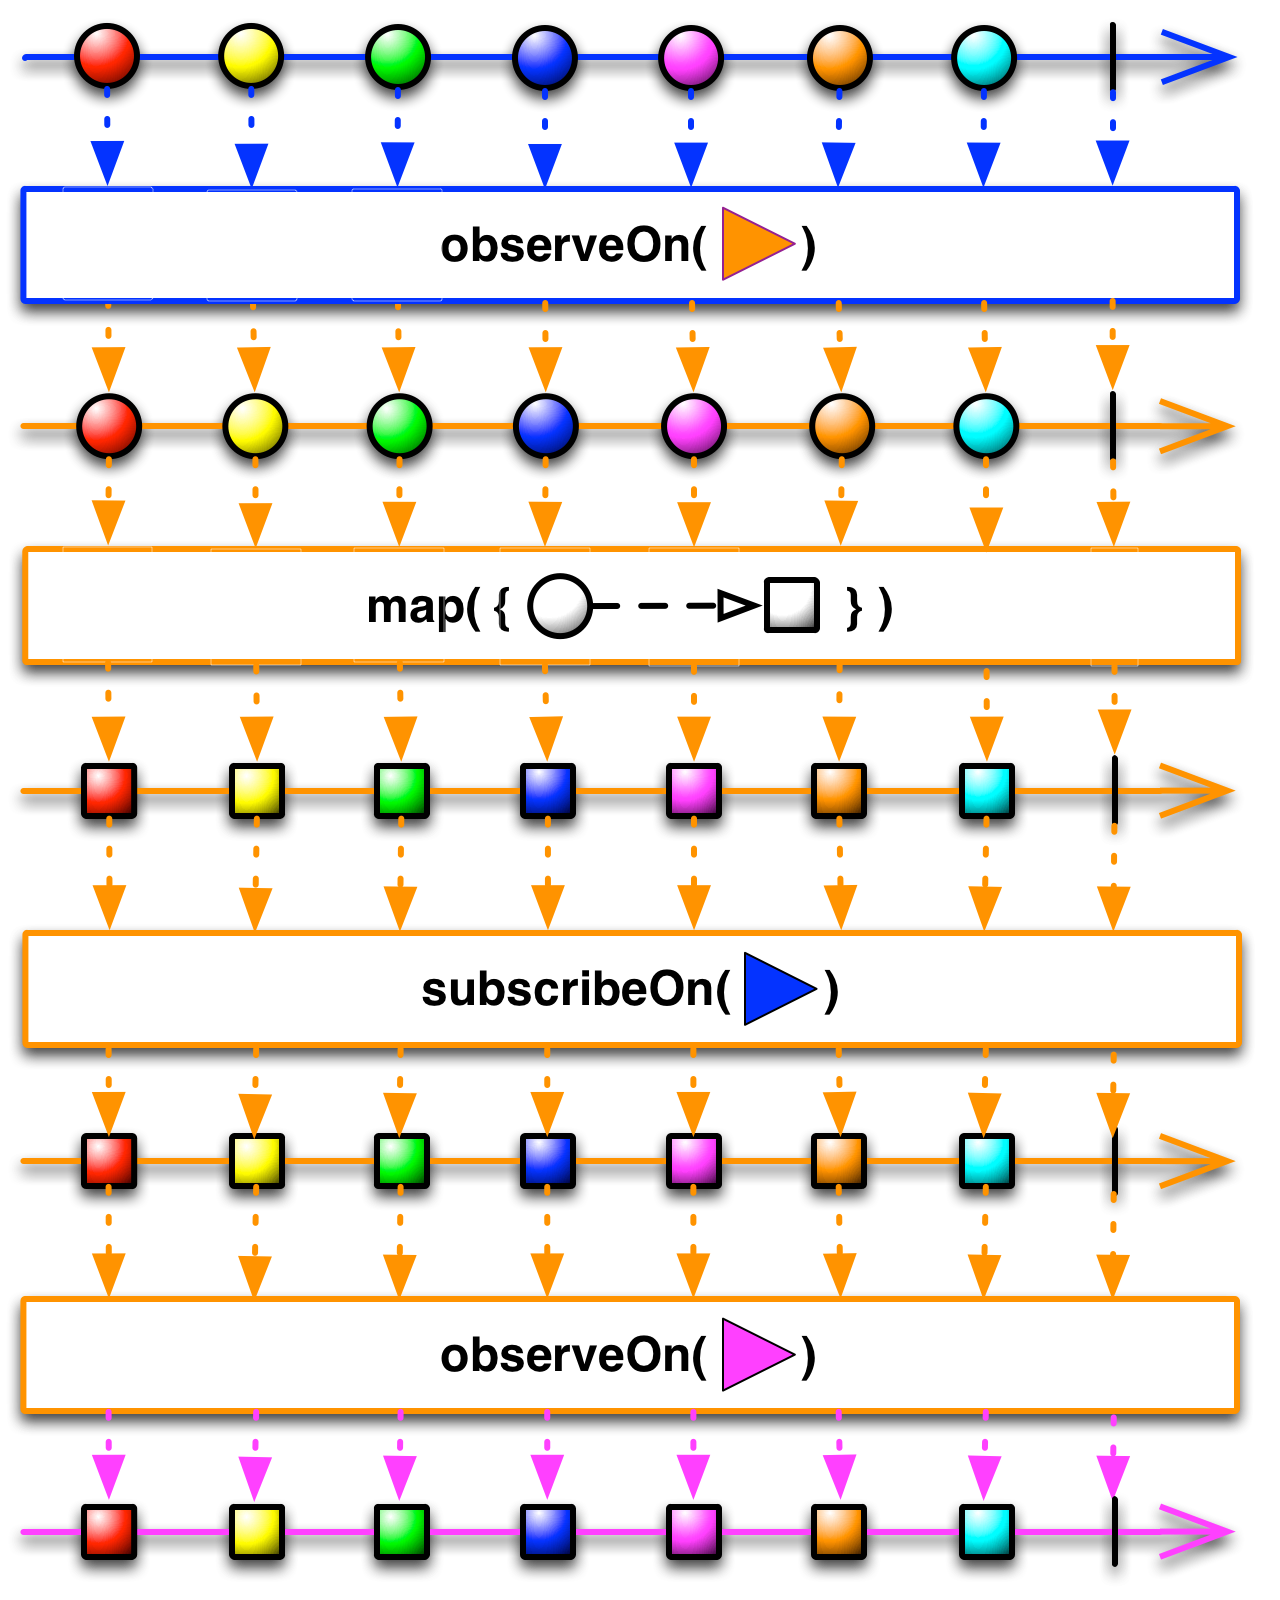
\includegraphics[width=10cm]{schedulers}
	\caption{Schemat ukazujący sposób przełączania między wątkami w środowisku reaktywnym\cite{scheduler}}
	\label{schedulers}
\end{figure}
Rysunek \ref{scheduler} przedstawia działanie przełączania między wątkami.
\pagebreak
\paragraph{Rodzaje planistów w implementacji RxSwift}
\subparagraph{CurrentThreadScheduler (Serial scheduler)}
Jednostka zadania, zaplanowywana jest do wykonania na bieżącym wątku. Czasami nazywany planistą trampolinowym. \\
Jeśli metoda CurrentThreadScheduler.instance.schedule(state) \{ \} jest wywoływana po raz pierwszy na jakimś wątku, to planowane zadanie zostanie wykonane natychmiastowo i zostanie utworzona ukryta kolejka, w której wszystkie rekursywnie zaplanowane zadania zostaną tymczasowo umieszczone.
\subparagraph{MainScheduler (Serial scheduler)}
Odsyła pracę do wykonania na główny wątek (MainThread). W przypadku, gdy metody zaplanowujące, wywoływane są już na głównym wątku to zadanie zostane wykonane natychmiastowo, bez planowania.\\
Najczęściej ten planista używany jest do wykonywania pracy związanej z interfejsem użytkownika (UI).
\subparagraph{SerialDispatchQueueScheduler (Serial scheduler)}
Odsyła pracę, która ma być wykonana z użyciem konkretnej szeregowej kolejki zadań typu dispatch\_queue\_t. Zapewnia, że nawet jeżeli w argumencie zostanie przesłana kolejka współbieżnych zadań to zostanie ona przekształcona do szeregowej kolejki zadań.\\
Planiści kolejkowi stosują pewne optymalizacje do metody observeOn.\\
Planista główny (Main Scheduler) jest instancją typu SerialDispatchQueueScheduler.
\subparagraph{ConcurrentDispatchQueueScheduler (Concurrent scheduler)}
Odsyłą pracę, która ma być wykonana z użyciem konkretnej współbieżnej kolejki  typu dispatch\_queue\_t. Można w argumencie przesłać również kolejkę typu szeregowego i nie powinno stanowić to problemu.\\
Ten planista jest odpowiedni, gdy jakaś praca powinna być wykonana w tle.
\subparagraph{OperationQueueScheduler (Concurrent scheduler)}
Odsyła pracę która ma być wykonana z użyciem konkretnej kolejki typu NSOperationQueue.\\
Ten planista jest odpowiedni do przypadków, gdzie musi zostać wykonana większa, bardziej wymagająca praca, w tle a użytkownik chce dostroić przebieg współbieżnych procesów używając do tego stałej maxConcurrentOperationCount.

\subsection{Zalety i wady podejścia reaktywnego} 
Programowanie reaktywne znacząco podnosi poziom abstrakcji kodu, dzięki czemu można skupić się na wzajemnych zależnościach między zdarzeniami, tak aby zdefiniować logikę biznesową, zamiast na zawiłościach i szczegółach implementacyjnych.\\
Korzyść ta jest szczególnie widoczna w przypadku nowoczesnych aplikacji webowych i mobilnych, które oferują bardzo dużą interakcję z użytkownikiem. Owa interakcja ma bezpośredni wpływ na dane i decyzje podejmowane w systemie. Na początku XXI wieku, interakcja z aplikacjami webowymi sprowadzała się najczęściej do zatwierdzenia długiego formularza, przesłania go do aplikacji serwerowej (backend) i po prostym przetwarzaniu, wysłania odpowiedzi spowrotem do klienta (frontend). Od tamtego czasu aplikacje wyewoluowały do działania bardziej w czasie rzeczywistym: zmodyfikowanie pola formularza może automatycznie spowodować zapis w aplikacji serwerowej; reakcje użytkowników serwisów społecznościowych (np. "like'i") na treści zamieszczane przez innych użytkowników są ze sobą połączone i również prezentowane w czasie rzeczywistym. 

\paragraph{Korzyści z użycia RxSwift (iOS)}
\subparagraph{Bindowanie } Za pomocą mechanizmu bindowania w RxSwift, możliwe jest połączenie zachowania elementów UI z emitowanymi sygnałami. Mechanizm ten doskonale uzupełnia podejście w architekturze MVVM. 
\subparagraph{Powtórzenia } Narzędzie szczególnie przydatne przy zapytaniach sieciowych do API. Niestabilne lub wolne połączenie z Internetem może być przyczyną wielu błędów. Dzięki operatorowi retry (opisanego w sekcji "Operatory reaktywne"), możliwe jest powtórzenie wykonania zapytania sieciowego, bez implementowania skomplikowanej logiki i przetrzymywania stanów połączenia.
\subparagraph{Delegaty } Możliwe jest wykluczenie używania wbudowanych mechanizmów delegatów na rzecz bindingu reaktywnego. Daje to dużą przejrzystość kodu. 
\subparagraph{Anulowanie } Czasami logika biznesowa wymaga, aby kosztowne operacje (zapytania sieciowe, przetwarzanie grafiki) mogły być anulowane w trakcie ich trwania. Przykładem może być tutaj pobranie tablicy zdjęć i nałożenie na nich filtra a następnie załadowanie do obiektu TableView. Z punktu widzenia User Experience, nie ma sensu załadowywanie wszystkich zdjęć jeśli tylko część z nich jest widoczna w danym momencie, albo gdy użytkownik przewija tabelę zbyt szybko. Z pomocą przychodzi tutaj dobra obsługa wielowątkowości i mechanizm anulowania i dealokowania sygnałów w RxSwift.
\subparagraph{Agregowanie zapytań sieciowych } Gdy istnieje potrzeba odpytania wielu serwisów webowych i zagregowania ich odpowiedzi, podejście reaktywne zdaje się być odpowiednim narzędziem. Bez względu na to czy odpytania te powinny odbywać się współbieżnie czy może od odpowiedzi jednego będzie zależało uruchomienie następnego. Dzięki wcześniej opisanym operatorom możliwe jest zaimplementowanie wielu zapytań sieciowych w dowolnej kombinacji i zależności. 
\paragraph{Wady podejścia reaktywnego}
\subparagraph{Wysoki próg wejścia } Idea paradygmatu reaktywnego nie jest trywialna. Osoba rozpoczynająca naukę tego podejścia, zmuszona jest przestawić myślenie na takie postrzegające każdy obiekt jako sygnał. Nieistotne są stany lecz przepływ danych i efekty uboczne. 
\subparagraph{Zarządzanie pamięcią } Większość implementacji paradygmatu reaktywne oferuje automatyczne mechanizmy zarządzania pamięcią. Niekiedy jednak użytkownik sam musi zadbać o taki aspekt jak dealokowanie obiektu Observable. W przypadku implementacji na platformie iOS przykładem może być obiekt TabBarController, który trzyma referencje do wszystkich kontrolerów reprezentujących zakładki. W związku z tym nie zostaną one zdealokowane nigdy w czasie działania programu. Należy zatem zadbać o to, by sygnały używane w projekcie nie zajmowały niepotrzebnie zasobów jeśli zdarzenia od nich nie są w danym momencie przetwarzane.
\subparagraph{Debugowanie } Działanie wielu sygnałów na różnych wątkach może utrudniać debugowanie w razie błędów. W przypadku wycieków pamięci niezbędne jest szczegółowe zbadanie podejrzanego sygnału i jego pracy na każdym z używanych wątków.
\subsection{Podejście praktyczne w implementacji na platformie iOS}
\paragraph{}Na podstawie przykładów\cite{examples} w tym paragrafie, ukazane zostało praktyczne podejście do tematu programowania reaktywnego, poprzez ich realizację w implementacji RxSwift.
\paragraph{Przykład 1 - stan przejściowy}
\subparagraph{}W czasie tworzenia programów działających asynchronicznie, można napotkać wiele problemów z przejściowymi stanami. Typowym przykładem jest tutaj pole wyszukiwania z autouzupełnianiem.\\
Chcąc stworzyć obiekt pola wyszukiwania z autouzupełnianiem, pierwszym problemem jaki zostanie napotkany to sytuacja, gdy użytkownik chcący wyszukać wyniki dla frazy "abc", wpisze literę "c" w polu wyszukiwania, podczas gdy zapytanie sieciowe dla treści "ab" jest już oczekujące i musi zostać anulowane. Co prawda bez użycia podejścia reaktywnego, problem nie jest trudny do rozwiązania. Wystarczy stworzyć dodatkową zmienną utrzymującą referencję do oczekującego zapytania sieciowego.\\
Kolejną sytuacją, którą trzeba obsłużyć to potencjalny błąd w procesie zapytania sieciowego. Należy wówczas zastosować często zagmatwaną logikę do powtórzenia całego procesu.\\
Ponadto idealną sytuacją byłoby, gdyby program zaczekał pewien czas zanim zapytanie sieciowe byłoby rzeczywiście realizowane. W końcu, nie jest porządanym, aby serwer był odpytywany za każdym razem, gdy użytkownik wpisze znak w polu wyszukiwania. Można próbować w tej sytuacji zastosować dodatkowy licznik czasu weryfikujący liczbę zapytań w czasie, tak aby nie przeciążyć serwera.\\
Pozostaje jeszcze kwestia, co powinno być wyświetlane w czasie wykonywania zapytania oraz co powinno być wyświetlone w przypadku błędu i to pomimo kilku prób.\\
Zaprogramowanie powyższego przykładu jest oczywiście możliwe bez podejścia reaktywnego, ale może wprowadzać niepotrzebne zawiłości.
O to jak powyższa logika może zostać zrealizowana przy użyciu RxSwift:
\begin{figure}[ht!]
	\centering
	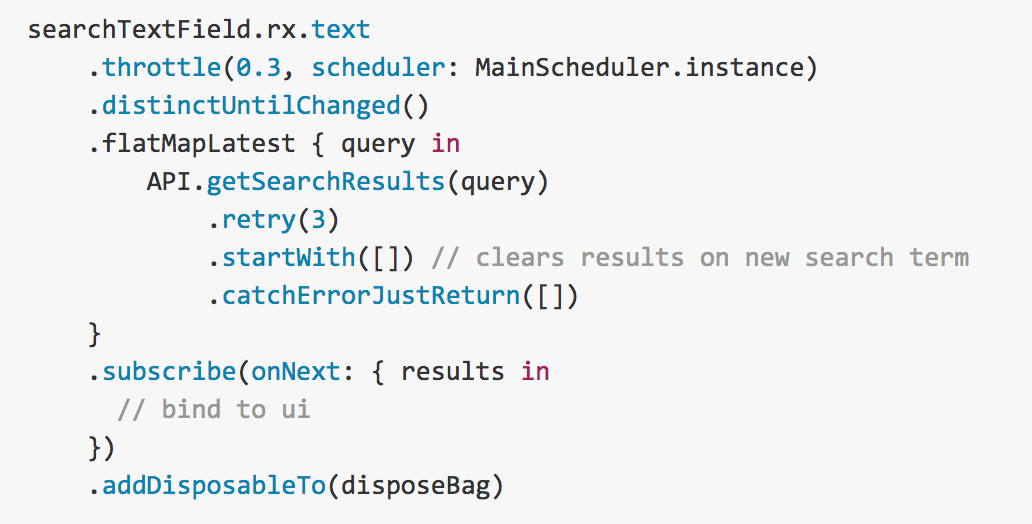
\includegraphics[width=15cm]{transientState}
	\caption{Przykładowy program realizujący powyższy przykład 1.\cite{transientState}}
	\label{transientState}
\end{figure}
\\\\\\\\\\\\\\
Jak widać na listingu \ref{transientState}, niepotrzebne są żadne dodatkowe flagi ani stany.
\paragraph{Przykład 2 - częściowe anulowanie}
\subparagraph{}Scenariuszem tego przykładu będzie następujący ciąg działań: ma nastąpić pobranie zestawu zdjęć z zewnętrznego adresu URL, następnie zdjęcia mają zostać zdekodowane i obłożone filtrem rozmywającym. Na koniec wyświetlane są w komórkach tabeli TableView.\\
Założenia: 
\begin{itemize}
	\item Całość procesu powinna być anulowana dla komórki wychodzącej z obszaru widoczności, tak aby nie zużywać pasma internetowego i czasu procesora na nakładanie filtru, jako że są to operacje kosztowne.
	\item Całość procesu nie powinna się rozpoczynać bezpośrednio w chwili, gdy komórka wejdzie obszar widoczności. Użytkownik może przewijać widok tabeli bardzo szybko, co powodowałoby uruchamianie wielu zapytań sieciowych, które natychmiastowo musiałyby zostać anulowane.
	\item Dobrą praktyką byłoby ograniczenie liczby współbieżnych operacji nakładania filtru na zdjęcia, bo jest to operacja kosztowna.
\end{itemize}
Oto w jaki sposób można zrealizować powyższą logikę z użyciem podejścia reaktynwego w RxSwift: 
\begin{figure}[ht!]
	\centering
	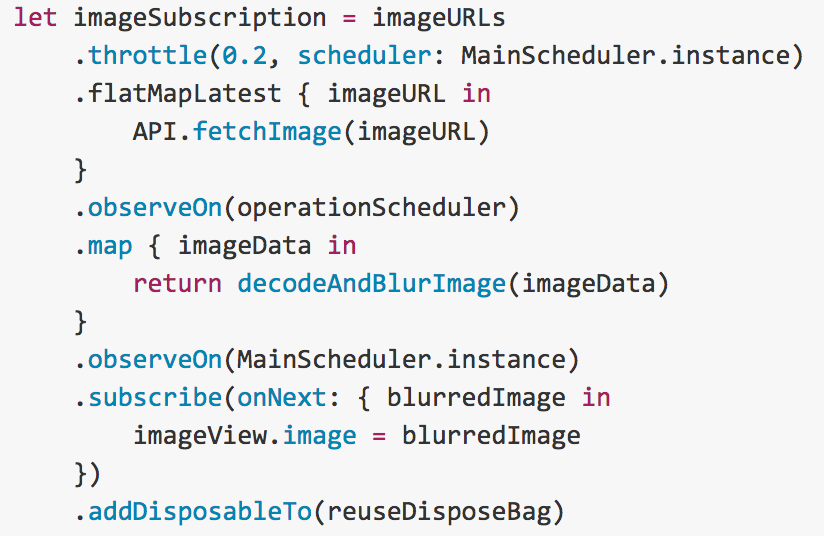
\includegraphics[width=12cm]{compositionalDisposal}
	\caption{Przykładowy program realizujący przykład 2.\cite{transientState}}
	\label{compositionalDisposal}
\end{figure}\\
Listing \ref{compositionalDisposal} ukazuje kod, który zrealizuje założenia oraz gdy obiekt imageSubscription zostanie zdealokowany, zapewni że wszystkie zależne od niego asynchroniczne operacje zostaną anulowane, i że żadne błędne obrazy nie będą połączone z interfejsem użytkownika.
\pagebreak
\paragraph{Przykład 3 - agregowanie zapytań sieciowych}
\subparagraph{}W tym przykładzie zostanie pokazana sytuacja, w której potrzebne jest zrealizowanie dwóch niezależnych zapytań sieciowych i zagregowanie ich wyników, gdy oba się zakończą. W tym celu, użyty zostanie operator \textbf{zip}.\\
W poniższym listingu można dostrzeć, że obsłużona została częsta sytuacja, w której odpowiedzi od API obsługiwane są na wątku w tle a binding tych odpowiedzi do interfejsu użytkownika powininen odbyć się na wątku głównym. Ten problem, rozwiązany został przy użyciu operatora \textbf{observeOn}.
\begin{figure}[ht!]
	\centering
	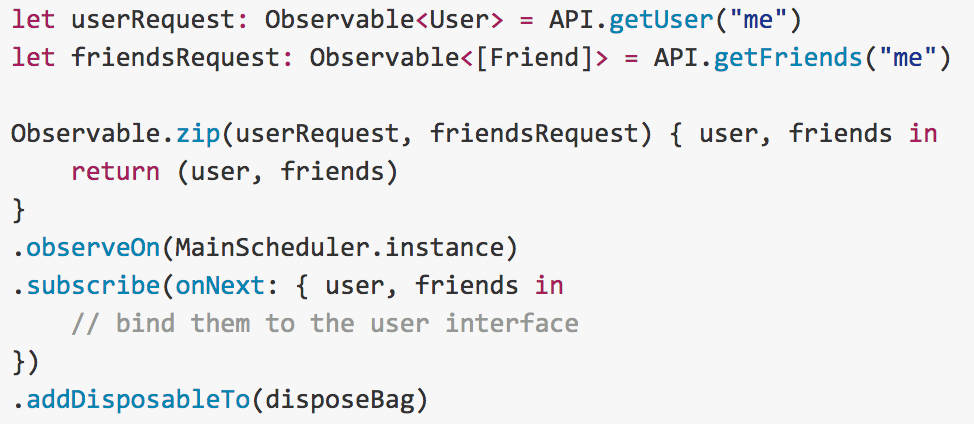
\includegraphics[width=14cm]{aggregatingNetworkRequests}
	\caption{Przykładowy program realizujący przykład 3.\cite{transientState}}
	\label{aggregatingNetworkRequests}
\end{figure}
Powyższy obrazek \ref{aggregatingNetworkRequests} przestawia sposób implementacji przykładu.
\chapter{PRACA WŁASNA}
\section{Czynności przygotowawcze}		
\paragraph{}Stworzenie aplikacji mobilnej było możliwe dzięki wykonaniu uprzednio czynności przygotowawczych. Do czynności tych należało: wybór środowiska programistycznego, instalacja bibliotek i frameworków, wstępna konfiguracja projektu oraz stworzenie repozytorium.
\subsection{Instalacja narzędzi}
\paragraph{}Program XCode jest jednym z niewielu dostępnych środowisk programistycznych na platformę iOS. Jest on darmowy i dostarczany wraz systemem MacOS. XCode posiada wbudowany kompilator LLVM oraz szereg przydatnych narzędzi tj. interface builder - graficzny edytor do tworzenia elementów interfejsu, dynamiczną kontrolę składni czy menedżer systemu kontroli wersji. Ze względu na powyższe właściwości użyto właśnie tego środowiska programistycznego.
Ponadto użyto narzędzia do rozwiązywania zależności - CocoaPods. Jest ono bardzo przydatne szczególnie przy instalacji bibliotek i frameworków do projektu.  
\subsection{Wstępna konfiguracja projektu}
\paragraph{}Podczas konfigurowania projektu w środowisku XCode istotne jest abyśmy stworzyli go z użyciem CoreData. Jest to baza danych środowiska iOS i może stanowić integralną część aplikacji.   
\subsection{Stworzenie repozytorium}
\paragraph{}Dostępnych jest wiele systemów kontroli wersji, ale najpopularniejszym z nich jest GIT. Zdecydowałem się na jego wykorzystanie, ponieważ jest dosyć prosty w użyciu a większość serwerów GITa jest darmowa. Użycie systemu typu GIT pozwoli mi na kontrolę postępów mojej pracy jak i na dokumentowanie jej. Oprócz tego użycia GITa powoduje, że błąd popełniony przeze mnie na dalszym etapie mogę odwrócić przywracając poprzedni stan projektu.
\pagebreak
\section{Budowa aplikacji właściwej}
\paragraph{}Ninejszy projekt powstawał w oparciu o niektóre elementy modelu kaskadowego\cite{modelKaskadowy} cyklu życia oprogramowania. Model ten stosowany jest często w praktyce do projektów o niewielkiej złożoności. Obejmuje następujące etapy:
\begin{itemize}
	\item Określenie wymagań
	\item Projektowanie systemu
	\item Implementacja i testowanie modułów
	\item Testowanie połączeń modułów i całości systemu 
	\item Użytkowanie i pielęgnacja
\end{itemize}
\subsection{Wymagania funkcjonalne}
\begin{itemize}
	\item Nawigacja pomiędzy zakładkami
	\item Wyszukiwanie filmu lub serialu i wyświetlenie wyniku w tabeli
	\item Podgląd szczegółów dot. filmu lub serialu tj. oceny użytkowników serwisu filmowego IMDB czy plakatu
	\item Możliwość dodania filmu bądź serialu do swojej bazy
	\item Możliwość oznaczenia filmu bądź serialu jako obejrzany i wystawienie mu oceny w swojej bazie
	\item Podgląd wszystkich dotychczas zapisanych filmów i seriali wraz z ocenami jeśli zostały nadane
	\item Możliwość wyświetlenia propozycji do obejrzenia z bazy zapisanych filmów i seriali w zależności od wprowadzonego przez użytkownika czasu 
\end{itemize}

\subsection{Wymagania niefunkcjonalne}
\begin{itemize}
	\item Spójność danych - dane podczas przesyłania nie mogą ulec zniekształceniu
	\item Szybkość transmisji - wszystkie operacje muszę odbywać się w czasie umożliwiającym płynne działanie aplikacji
	\item Stabilność połączenia - aplikacja, do prawidłowego działania, wymaga stabilnego połączenia internetowego 
	\item Ograniczenie liczby zapytań API do minimum
	\item Brak zasobożerności aplikacji pomimo używania przez niej wielu wątków 
\end{itemize}
\subsection{Diagram przypadków użycia aplikacji}
\begin{figure}[ht!]
	\centering
	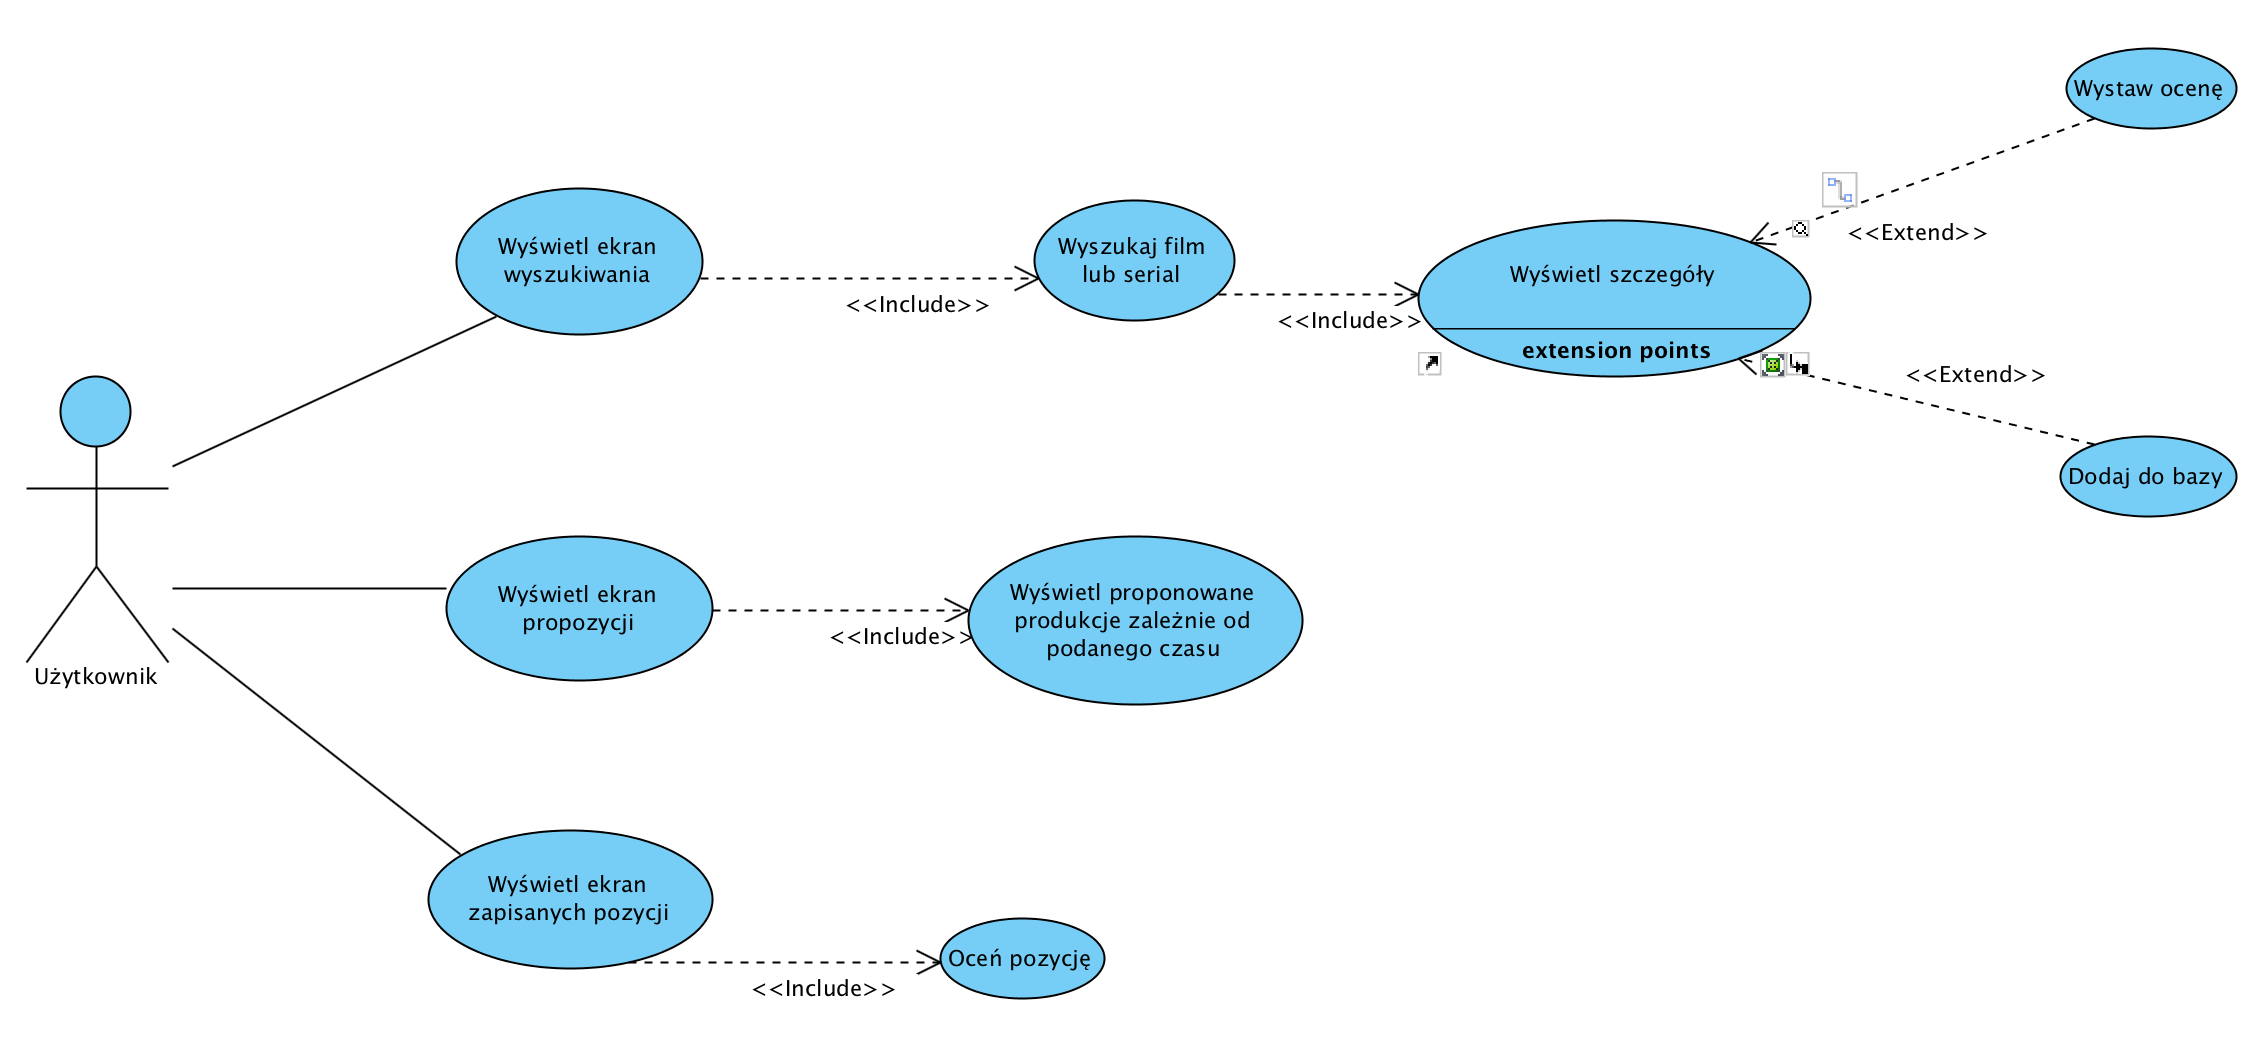
\includegraphics[width=17cm]{useCase'y}
	\caption{Schemat przypadków użycia 
		\textit{źródło:własne }}
	\label{useCase'y}
\end{figure}
\subparagraph{}Schemat \ref{useCase'y} przedstawia ogólne przypadki użycia aplikacji mobilnej. Użytkownik może wykonywać nastepujące czynności:
\begin{itemize}
	\item Wyświetlić ekran wyszukiwania
	\item Wyszukać film lub serial
	\item Wyświetlić szczegóły dot. znalezionego filmu lub serialu
	\item Wystawić ocenę znalezionemu filmowi lub serialowi
	\item Zapisać w bazie znaleziony film lub serial
	\item Wyświetlić ekran propozycji
	\item Wyświetlić proponowane pozycje do obejrzenia przy uwzględnieniu czasu wprowadzonego przez użytkownika
	\item Wyświetlić ekran zapisanych pozycji
	\item Ocenić zapisane pozycje
\end{itemize}
\subsection{Baza danych}
\paragraph{}W bazie danych przetrzymywane są informacje o zapisanych przez użytkownika pozycjach reprezentujących film lub serial, które użytkownik chciałby obejrzeć. Baza ta nie jest skomplikowana i nie w wymaga więcej niż modelu jednej encji. Encja ta wystarcza do przechowywania żądanych informacji i nie istnieją relacje z innymi encjami.
\begin{figure}[ht!]
	\centering
	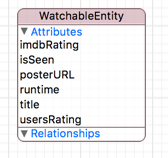
\includegraphics[width=7cm]{watchableEntity}
	\caption{Diagram bazy danych 
		\textit{źródło:własne }}
	\label{watchableEntity}
\end{figure}
\subparagraph{}Na diagramie \ref{watchableEntity}, można zobaczyć encję posiadającą następujące atrybuty:
\begin{itemize}
	\item \textbf{imdbRating} - reprezentuje ocenę użytkowników serwisu IMDB
	\item \textbf{isSeen} - binarna wartość typu Bool, określająca czy użytkownik obejrzał już daną pozycję  
	\item \textbf{posterURL} - zewnętrzny adres URL informujący o tym skąd można pobrać grafikę dla danego filmu lub serialu
	\item \textbf{runtime} - reprezentuje czas trwania filmu lub serialu, brany pod uwagę przy mechanizmie proponowania
	\item \textbf{title} - reprezntuje tytuł pozycji
	\item \textbf{userRating} - ocena pozycji, wystawiona przez użytkownika aplikacji 
\end{itemize}
\newpage

\begin{landscape}
	\subsection{Diagram wybranych klas}
	\begin{figure}[ht!]
		\centering
		\includegraphics[width=26cm]{diagramKlas}
		\caption{Diagram klas
			\textit{źródło:własne}}
		\label{diagramKlas}
	\end{figure}
\end{landscape}
\subsection{Opis wybranych klas}
\begin{itemize}
	\item Klasa \textbf{AppDelegate} - główna klasa programu, tworzona automatycznie. Implementuje metody interfejsu UIApplicationDelegate, który jest odpowiedzialny za obsługe metod wywoływanych przez singleton UIApplication w odpowiedzi na ważne zdarzenia w cyklu życia aplikacji. Te ważne zdarzenia to m. in. zmiany stanu aplikacji takie jak przejście aplikacji w background, przejście w foreground, obsługa notyfikacji, interakcja z innymi aplikacjami w systemie czy interakcja z samym systemem iOS.
	\item Klasa \textbf{CoreDataStack} -  reprezentuje menedżera bazy danych CoreData. Jej metody pozwalają na pobranie bieżącego kontekstu, czyli stanu danych i relacji w bazie danych oraz zapisanie tego kontekstu.
	\item Klasa \textbf{WatchableEntity} - reprezentuje model encji bazodanowej. Jej metoda pozwala na wykonanie zapytania bazodanowego a jej pola reprezentują poszczególne atrybuty encji.
	\item Klasa \textbf{SearchForMovieViewController} - kontroler widoku wyszukiwania produkcji. Jej atrybutami są elementy interfejsu użytkownika t.j. tabela czy pasek wyszukiwania, który jest tutaj obsługiwany reaktywnie. Ponadto korzysta z modelu wyszukiwania produkcji w celu wyświetlenia znalezionych wyników. Nie posiada informacji o tym w jaki sposób przebiega proces wyszukiwania. 
	\item Klasa \textbf{MovieDetailsController} - kontroler widoku szczegółów na temat znalezionej produkcji. Odpowiedzialny jest za operacje interfejsu użytkownika takie jak pobranie obrazka czy wyświetlenie oceny znalezionego filmu lub serialu. Komunikuje się tylko z modelem MovieDetailsViewModel za pośrednictwem interfejsu MovieDetailsViewModelType, aby otrzymywać informacje na temat danych do wyświetlenia.
	\item Klasa \textbf{MovieDetailsViewModel} - stanowi model widoku dla klasy kontrolera poprzednio opisanego. Implementuje metody i pola interfejsu MovieDetailsViewModelType. Odpowiedzialna jest za reaktywne zmiany modelu widoku takie jak blokowanie/odblokowywanie możliwości kliknięcia przycisków, podawanie do kontrolera danych do wyświetlenia ze znalezionej produkcji, przygotowanie modelu widoku oceny filmu czy zapisanie pozycji w bazie danych. 
	\item Enumerator \textbf{OMDB} - implementuje metody i pola wymagane przez interfejs Mappable, potrzebny do działania modułu Moya odpowiedzialnego za zapytania sieciowe w sposób reaktywny. Enumerator ten odpowiedzialny jest za dostarczenie adresów URL wszystkich używanych endpointów API, metod odpytania, sposobu kodowania odpowiedzi oraz przykładowy model zwracanych przez API danych.   
	\item Klasa \textbf{WatchableFinderModel} - model wyszukiwania filmów i seriali. Izoluje logikę i sposób odpytywania API od reszty klas. Korzysta z dostarczanego przez framework Moya providera zależnego od uprzednio opisanego enumeratora dostarczającego wszystkich potrzebnych danych. Jego metody generują sygnały będące wynikiem odpytywania API o zadany tytuł. 
	\item Klasa \textbf{Watchable} - model danych reprezentujących znaleziony przez API film lub serial. Implementuje interferjs Mappable, który odpowiedzialny jest za przeprowadzenie próby zmapowania otrzymanego w odpowiedzi (od API) obiektu typu JSON na obiekt typu Mappable.
\end{itemize}
\pagebreak
\subsection{Opis użytych bibliotek i frameworków}
\paragraph{}Stworzenie projektu aplikacji mobilnej wymagało zastosowania niezbędnych bibliotek. Zgodnie z tematem pracy, aplikacja powinna opierać się o paradygmat reaktywny, który został zaimplementowany dzięki stworzonym do tego, zewnętrznym modułom i bibliotekom. \\
Poniżej, zostały przedstawione użyte moduły i ich krótka charakterystyka:
\begin{itemize}
	\item  \textbf{CocoaPods} - menedżer zależności w projektach XCode. Dzięki niemu, możliwe jest określenie zależności w projekcie dzięki prostemu plikowi textowemu \textbf{Podfile}. CocoaPods rekursywnie rozwiązuje zależności pomiędzy użytymi bibliotekami, wyszukuje kod źródłowy dla wszystkich zależności oraz tworzy i utrzymuje obszar roboczy w celu budowania projektu XCode (plik .xcworkspace).\cite{cocoaPods}
	\item  \textbf{UIKit} - dostarcza niezbędnej infrastruktury potrzebnej do skonstruowania i zarządzania aplikacją na platformie iOS i tvOS. Jest to framework zapewniający architekturę okna i widoku do zarządzania interfejsem użytkownika w aplikacji. Ponadto służy do obsługi zdarzeń potrzebnych do odpowiedzi na reakcje użytkownika oraz dostarcza modelu aplikacji odpowiedzialnego za działanie pętli głównej programu i interakcji z systemem.\cite{UIKit}
	\item  \textbf{CoreData} - graf obiektów\cite{objectGraph} i framework warstwy modelu zapewniający trwałość tych obiektów.
	Pozwala, aby dane zorganizowane w model relacyjny encja-atrybut, były serializowane do postaci XML, binarnej lub zasobów SQLite.
	Danymi można zarządzać używając wysokopoziomowych obiektów reprezentujących encje i ich relacje. CoreData zarządza wersjami zserializowanymi, zapewniając cykl życia obiektu i możliwość zarządzania grafem obiektów włączając w to trwałość tych obiektów.\\
	CoreData jest bezpośrednim interfejsem SQLite izolującym programistę od działającego "pod spodem" języka SQL.
	
	\item  \textbf{RxSwift} - implementacja biblioteki .NET Reactive Extensions w języku Swift na platformę iOS/macOS. Jest to próba przeportowania tak wielu konceptów z oryginalnej biblioteki Rx jak to tylko możliwe. Głównym zamierzeniem RxSwift jest umożliwienie łatwej kompozycji asynchronicznych operacji i strumieni zdarzenie/dane.
	
	\item  \textbf{RxCocoa} - nakładka na frameworki Cocoa i Cocoa Touch, rozszerzająca możliwości dostarczane przez nie (obiekty UI i ich obłsuga) o reaktywne zachowanie w oparciu o framework RxSwift.  
	\item  \textbf{RxOptional} - rozszerzenie RxSwift dla obiektów opcjonalnych w Swift, pozwalające na ich reprezentację w podejściu reaktywnym.
	\item  \textbf{Moya} - biblioteka stanowiąca nakładkę reaktywną na framework Alamofire\cite{alamofire} umożliwiający izolację logiki odpowiedzialnej za wszelkie operacje sieciowe. Dzięki jej użyciu możliwe jest przekształcenie architektury obsługi operacji sieciowych zgodnie z poniższym schematem:
	\begin{figure}[ht!]
		\centering
		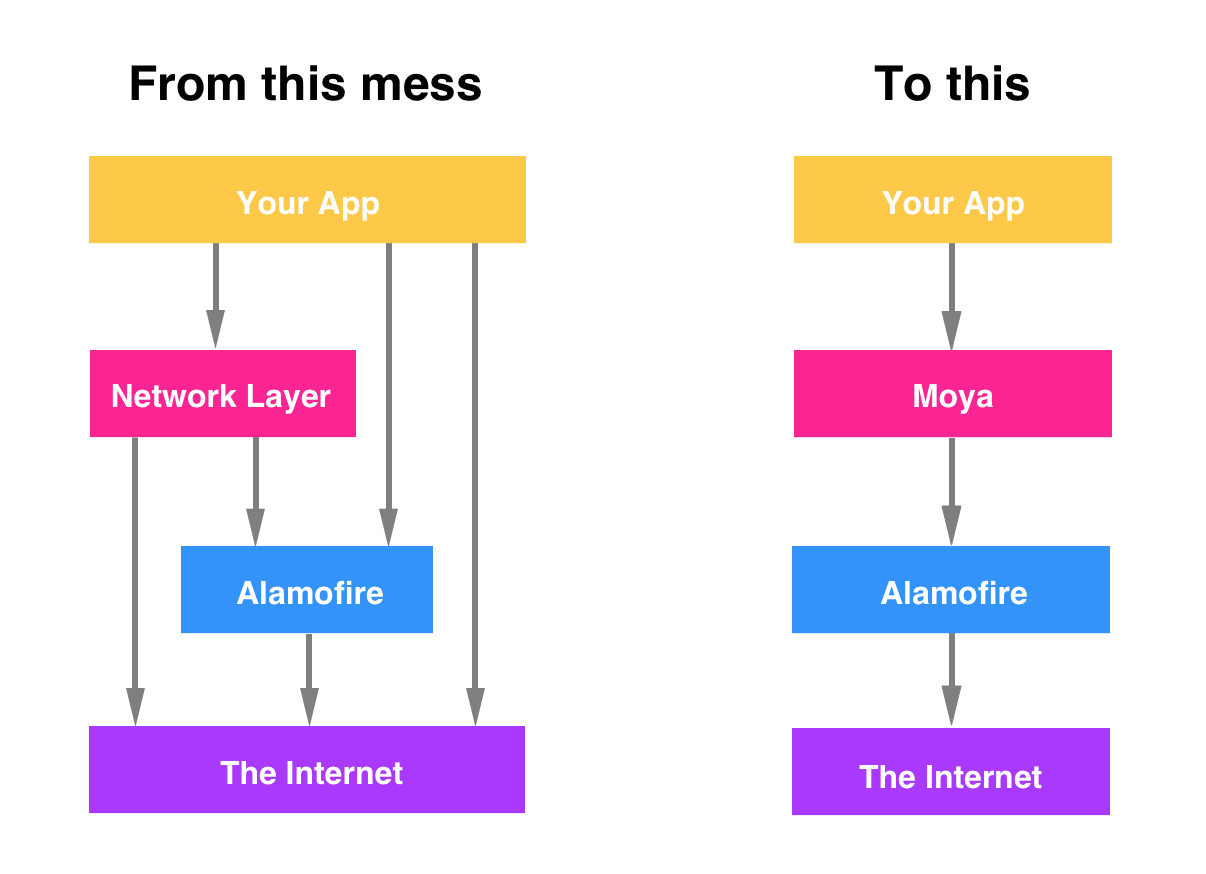
\includegraphics[width=13cm]{moyaDiagram}
		\caption{Przekształcenie logiki zapytań sieciowych dzięki Moya\cite{moyaScheme}}
		\label{moyaDiagram}
	\end{figure}
	Powyższy obrazek \ref{moyaDiagram} przedstawia architekturę aplikacji po zastosowaniu biblioteki Moya.
	\item  \textbf{Moya\_ModelMapper} - biblioteka stanowiąca nakładkę dla frameworku Mapper\cite{mapper} ułatwiającego konwersję JSON do silnie typowanych obiektów Swift. Moya\_ModelMapper dostarcza potrzebnych bindingów do biblioteki Moya do łatwiejszej serializacji obiektów JSON przy użyciu RxSwift.
\end{itemize}
\pagebreak
\subsection{Zastosowana architektura}
\paragraph{}Wybranie właściwej architektury w projekcie było niezbędne, aby w pełni ukazać co oferuje programowanie reaktywne w języku Swift. 
\paragraph{MVC}czyli Model View Controller jest najczęściej stosowanym podejściem jeśli chodzi o aplikacje na iOS lecz nie zawsze jest to podejście właściwe. \\
Typowo, architektura ta powinna się sprowadzać do poniższego schematu:
	\begin{figure}[ht!]
	\centering
	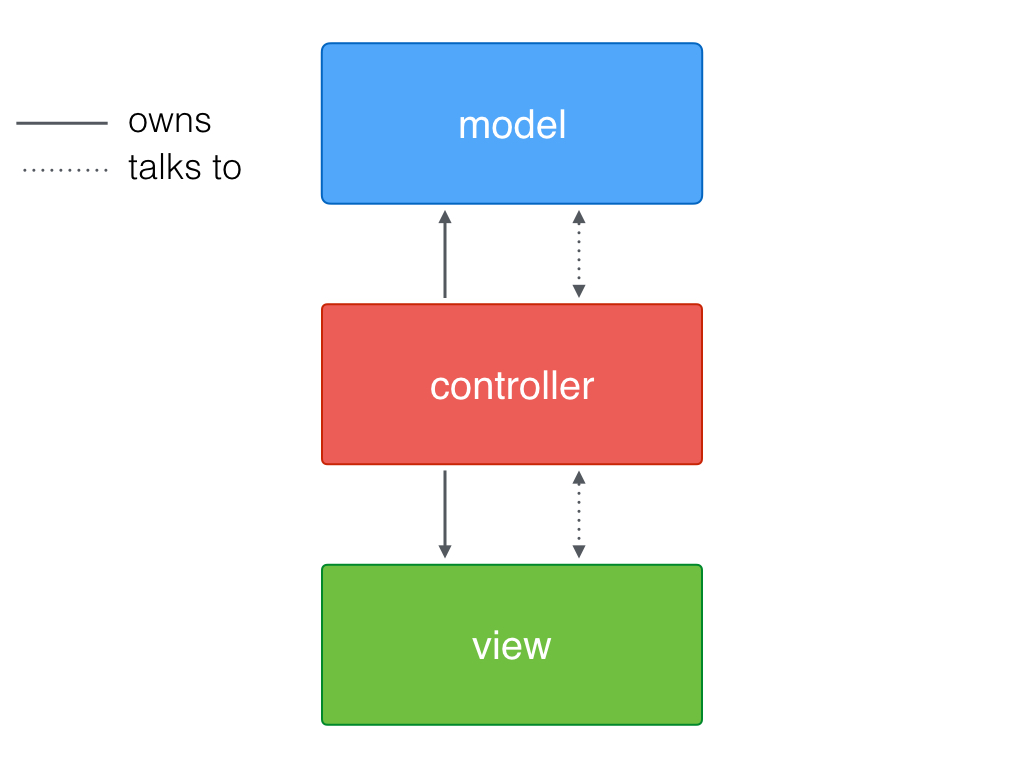
\includegraphics[width=13cm]{MVC}
	\caption{architektura MVC\cite{MVC}}
	\label{MVC}
\end{figure}\\
Niestety, role poszczególnych komponentów w tej architekturze (rys. \ref{MVC}) nie zawsze są jasno określone i tak np. typowe zadanie formatowania daty nie pasuje jako rola widoku ani tym bardziej modelu, dlatego staje się wówczas odpowiedzialnością kontrolera. Wiele tego typu zadań zostaje rozwiązywane właśnie w obszarze kontrolera co powoduje poważne konsekwencje takie jak rozrost kontrolerów, trudności w testowaniu czy niemożność ich ponownego użycia w innych częściach aplikacji.
\paragraph{}Z powyższych powodów, architekturą wybraną do zaprojektowania ninejszej aplikacji został \textbf{MVVM}, czyli \textbf{Model-View-ViewModel}, który w środowisku iOS można sprowadzić do poniższego schematu:
  	\begin{figure}[ht!]
  	\centering
  	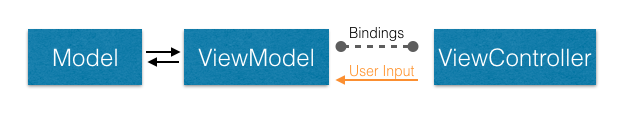
\includegraphics[width=13cm]{rxMVVM}
  	\caption{architektura MVVM\cite{rxMVVM}}
  	\label{rxMVVM}
  \end{figure}
\subparagraph{}W powyższej architekturze (rys.\ref{rxMVVM}) ViewModel stoi pomiędzy modelem a kontrolerem i dostarcza danych kontrolerowi, które powinien wyświetlić w widoku. Dzięki temu ViewController nie ma już bezpośredniego dostępu do modelu. Poprzednio rozpatrywane, typowe zadanie formatowania daty zostanie zlecone właśnie do ViewModelu, który przygotuje odpowiednio dane i już sformatowane, poda dalej do kontrolera.
\\Nie należy jednak oczekiwać od ViewModelu, aby wiedział w jaki sposób dane są wyświetlane przez ViewController. 
\subparagraph{}Z racji, że w powyżej przedstawionej architekturze, ViewModel "nie wie" nic o kontrolerze, komunikacja między tymi komponentami odbywa się na zasadzie nasłuchiwania. Kontroler przy pomocy reaktywnych bindingów obserwuje zmiany w ViewModelu i na tej podstawie reaguje, wyświetlając odpowiednie elementy interfejsu użytkownika, wykorzystując w ten sposób potencjał programowania reaktywnego. 
\pagebreak
\subsection{Prezentacja aplikacji}
\paragraph{}Główne funkcje aplikacji prezentowane są w widokach wybieranych spośród trzech zakładek paska dolnego.
\subparagraph{}\textbf{Widok wyszukiwania filmu/serialu}
\begin{figure}[ht!]
	\centering
	\includegraphics[width=6cm]{SearchVC}
	\caption{Widok wyszukiwania
		\textit{źródło:własne}}
	\label{SearchVC}
\end{figure}\\
W widoku \ref{SearchVC}, możliwe jest kliknięcie paska wyszukiwania i wpisywanie tytułu. Wprowadzany z klawiatury ciąg znaków przetwarzany jest w sposób reaktywny z użyciem operatora \textbf{debounce}. Ma to duże znaczenie, ponieważ użytkownik nie musi potwierdzać chęci wyszukiwania w żaden sposób. odbywa się to automatycznie. Należy jednak zwrócić uwagę, że zapytania sieciowe kierowane do API nie są wysyłane z każdą wprowazoną literą. Dzięki operatorowi debounce, możliwe jest spokojne wpisanie całości tytułu a po upłynięciu zadanego interwału czasowego (tutaj kilkadziesiąt milisekund), rozpocznie się proces wysyłania zapytania do API.\\
Odnaleziona pozycja wyświetlana jest natychmiastowo w chwili znalezienia.
\subparagraph{}\textbf{Widok szczegółów filmu/serialu}
\begin{figure}[ht!]
	\centering
	\subfloat[]{}
	\includegraphics[width=5cm]{addToMyBaseEnabled}
	\quad
	\subfloat[]{}
	\includegraphics[width=5cm]{alreadyInBase}
	\caption{Widok szczegółów  filmu/serialu}
	\label{watchableDetails}
\end{figure}\\
Na widoku \ref{watchableDetails}, prezentowane są szczegóły dotyczące znalezionej pozycji. Widoczny jest plakat danej produkcji oraz jej ocena wystawiona przez użytkowników serwisu IMDB. Ponadto użytkownik ma możliwość dodania filmu/serialu do swojej bazy jeżeli jeszcze tego nie zrobił. Lokalna baza danych przeszukiwana jest w celu odnalezienia bieżącej produkcji i na tej podstawie decyduje się o sposobie wyświetlenia przycsisku.
\pagebreak
\subparagraph{}\textbf{Widok propozycji}
\begin{figure}[ht!]
	\centering
	\subfloat[]{}
	\includegraphics[width=5cm]{giveMeProposition}
	\quad
	\subfloat[]{}
	\includegraphics[width=5cm]{propositions}
	\caption{Widok proponowania pozycji do obejrzenia}
	\label{proposition}
\end{figure}\\
Widok \ref{proposition} prezentuje ekran propozycji. Użytkownik wybiera jedną z czterech opcji czasowych. Po zaznaczeniu opcji, kliknięcie przycisku spowoduje przeszukanie bazy zapisanych pozycji pod kątem filmów lub seriali spełniających wymóg czasowy, to znaczy, że czas ich trwania nie będzie dłuższy od czasu wybranego przez użytkownika. Ponadto przez filtr nie przejdą filmy i seriale już obejrzane (a przez to ocenione). 
\pagebreak
\subparagraph{}\textbf{Widok oceniania}
\begin{figure}[ht!]
	\centering
	\subfloat[]{}
	\includegraphics[width=5cm]{savedProductions}
	\quad
	\subfloat[]{}
	\includegraphics[width=5cm]{ratingVC}
	\caption{Widok oceniania zapisanych w bazie produkcji}
	\label{rating}
\end{figure}\\
W widoku \ref{rating} zaprezentowany jest ekran oceniania zapisanych filmów i seriali. Użytkownik ma możliwośc przeglądnięcia jakie filmy i seriale zapisał do swojej bazy. Przy tych, które zostały ocenione, wyświetlana jest wartość liczbowa reprezentująca jego ocenę. Kliknięcie w dowolną zapisaną w bazie produkcje, przenosi użytkownika do ekranu wystawienia oceny. Wartość wybierana jest przez przesuwanie paska. Przyciśnięcie przycisku powoduje zapisanie oceny do bazy. 
\chapter{PODSUMOWANIE}
\paragraph{}Celem niniejszej pracy było zgłębienie tematu programowania reaktywnego oraz zaprojektowanie i zbudowanie aplikacji mobilnej na system iOS w oparciu o omawiane zagadnienia.\\
Istnieje wiele implementacji tego podejścia, na różne języki programowania w tym kilka dla omawianego w tej pracy Swifta. Są to m.in.:RxSwift, Reactive Cocoa czy Reactive Swift. Jednakże wszystkie implementacje podejścia reaktywnego bazują na tej samej idei. Dzięki temu nie ma większego znaczenia ani to w jakim języku się tworzy ani to, przy użyciu której biblioteki programowania reaktywnego.
\subparagraph{}W części teoretycznej, została zawarta duża liczba rysunków i schematów. Zostało to podyktowane specyfiką omawianego tematu. Próg zrozumienia idei programowania reaktywnego, postawiony został dość wysoko. Z tego powodu, dla lepszego przyswojenia poruszanych zagadanień, załączono dużo grafik mających na celu ułatwienie i zobrazowanie mechanizmów reaktywnych.\\
Pomimo iż programowanie reaktywne nie jest tematem kompletnie nowym, to udokumentowanie go dla języka Swift pozostawia wiele do życzenia. Z tego powodu, w niniejszej pracy posiłkowano się dokumentacją do takich platform jak .NET Microsoftu, jak również Java czy JavaScript. 
\subparagraph{}Część praktyczna również stanowiła duże wyzwanie. Za cel, postawiono stworzenie aplikacji mobilnej w oparciu o architekturę MVVM. Po połączeniu z podejściem reaktywnym, wynikiem stało się zadanie o dużym stopniu trudności od strony programistycznej (wysoki poziom abstrakcji i kompletnie inny sposób myślenia) jak i od strony dostępności wiedzy (mała dokumentacja).
Należy również zaznaczyć, że projekt aplikacji stworzony został przy użyciu najnowszej implementacji języka Swift (iteracja 3.0) wprowadzającej szereg zmian w API. W czasie powstawania aplikacji, wykorzystywane biblioteki do programowania reaktywnego, uległy zmianie i aktualizacji do najnowszych implementacji.\\
Pomimo powyższych trudności, udało się stworzyć aplikację mobilną, opartą o architekturę MVVM i implementującą podejście reaktywne.
\subparagraph{}Podsumowując: programowanie reaktywne wraz z architekturą MVVM na platformy mobilne stanowi nielada wyzwanie. Jednakże jest to podejście wykorzystujące cały potencjał urządzeń mobilnych i zdecydowanie warte podjęcia próby wdrożenia w projektach komercyjnych. Jest polecane przez doświadczonych i znanych w branży programistów i coraz więcej firm decyduje się na zastosowanie tego właśnie podejścia\cite{reactivexio}.
\begin{thebibliography}{50}
\bibitem{MicrosoftRx} https://msdn.microsoft.com/en-us/library/hh242985(v=vs.103).aspx
\emph{- informacje na temat Reactive Extensions od Microsoft}

\bibitem{swiftHistory} https://developer.apple.com/swift/blog/?id=14
\emph{- historia języka Swift}

\bibitem{swiftOpensource} https://developer.apple.com/swift/blog/?id=34
\emph{- Swift jako język opensource}

\bibitem{swiftObjcDiff} https://redwerk.com/blog/10-differences-objective-c-swift
\emph{- Różnice między Swiftem a Objective - C}

\bibitem{pureDarwin} www.puredarwin.com 
\emph{ - informacje o systemie Darwin}

\bibitem{openGroup} www.opengroup.org \emph{ - informacje o systemach unixowych}

\bibitem{introToRx} https://gist.github.com/staltz/868e7e9bc2a7b8c1f754
\bibitem{subjects} http://reactivex.io/documentation/subject.html
\bibitem{operators}http://reactivex.io/documentation/operators.html
\bibitem{marbles}http://rxmarbles.com/
\bibitem{scheduler}http://reactivex.io/documentation/scheduler.html
\bibitem{transientState}https://github.com/ReactiveX/RxSwift/blob/master/Documentation/Why.md
\bibitem{moyaScheme}https://github.com/Moya/Moya/blob/master/web/diagram.png
\bibitem{MVC}https://cocoacasts.com/what-is-wrong-with-model-view-controller/
\bibitem{rxMVVM}https://medium.cobeisfresh.com/implementing-mvvm-in-ios-with-rxswift-updated-for-swift-2-51cc3ef7edb3\#.47mux55lq


\bibitem{XNUkernel} https://developer.apple.com/library/content/documentation/MacOSX/Conceptual/OSX\_Technology\_Overview/SystemTechnology/SystemTechnology.html\#//apple\_ref/doc/uid/TP40001067-CH207-BCICAIFJ
\emph{ - opis jądra systemu MacOS i iOS}

\bibitem{iphoneOSX} https://web.archive.org/web/20071006005308/http://www.apple.com/iphone/features/index.html\#macosx
\emph{ - informacje o pierwszym systemie na iPhone}

\bibitem{iphoneSDK} https://web.archive.org/web/20071020040652/http://www.apple.com/hotnews
\emph{ - informacja o stworzeniu i udostępnieniu iPhone SDK}

\bibitem{iphone3GappStore} http://www.apple.com/pr/library/2008/07/10iPhone-3G-on-Sale-Tomorrow.html
\emph{ - informacje o iPhone 3G i powstaniu usługi App Store}

\bibitem{iphoneOS3} http://www.apple.com/pr/library/2009/06/08Apple-Announces-the-New-iPhone-3GS-The-Fastest-Most-Powerful-iPhone-Yet.html
\emph{ - system iPhone 3.0 i implementacja podstawowych funkcjonalności}

\bibitem{ios4}http://www.apple.com/pr/library/2010/04/08Apple-Previews-iPhone-OS-4.html
\emph{ - informacje o systemie iOS 4}

\bibitem{ios5}http://www.apple.com/pr/library/2011/10/04Apple-Launches-iPhone-4S-iOS-5-iCloud.html
\emph{ - informacje o systemie iOS 5}

\bibitem{ios6}http://www.apple.com/pr/library/2012/06/11Apple-Previews-iOS-6-With-All-New-Maps-Siri-Features-Facebook-Integration-Shared-Photo-Streams-New-Passbook-App.html
\emph{ - informacje o systemie iOS 6}

\bibitem{ios7}http://www.apple.com/pr/library/2013/06/10Apple-Unveils-iOS-7.html
\emph{ - informacje o systemie iOS 7}

\bibitem{ios8}http://www.apple.com/pr/library/2014/06/02Apple-Releases-iOS-8-SDK-With-Over-4-000-New-APIs.html
\emph{ - informacje o systemie iOS 8}

\bibitem{ios9}http://www.apple.com/pr/library/2015/06/08Apple-Previews-iOS-9.html
\emph{ - informacje o systemie iOS 9}

\bibitem{compatibility}https://github.com/apple/swift-evolution/blob/master/proposals/0005-objective-c-name-translation.md
\emph{ - informacje o poprawieniu kompatybilności Swift z Objective-C}

\bibitem{ios10}http://www.apple.com/pr/library/2016/06/13Apple-Previews-iOS-10-The-Biggest-iOS-Release-Ever.html
\emph{ - informacje o systemie iOS 10}

\bibitem{beginningOfRx} Czaplicki, Evan (Apr 2012), Elm: Concurrent FRP for Functional GUIs (PDF) (thesis), Harvard
\emph{ - pierwsze wzmianki o programowaniu reaktywnym}

\bibitem{rxMicrosoftYear} http://www.introtorx.com/content/v1.0.10621.0/00foreword.html
\emph{ - wypuszczenie biblioteki Reactive Extensions}

\bibitem{rxDesignGuideline} https://go.microsoft.com/fwlink/?LinkID=205219
\emph{ - wytyczne projektowe paradygmatu reaktywnego}

\bibitem{examples}https://github.com/ReactiveX/RxSwift/blob/master/Documentation/Why.md
\emph{ - przykłady użycia RxSwift}

\bibitem{modelKaskadowy} http://zasoby.open.agh.edu.pl/\~10sdczerner/page/model\_kaskadowy.html
\emph{ - model kaskadowy cyklu życia oprogramowania}

\bibitem{cocoaPods} https://github.com/CocoaPods/CocoaPods
\emph{ - opis menedżera zależności CocoaPods}

\bibitem{UIKit}https://developer.apple.com/reference/uikit
\emph{ - opis frameworku UIKit}

\bibitem{objectGraph} https://developer.apple.com/library/content/documentation/General/Conceptual/DevPedia-CocoaCore/ObjectGraph.html
\emph{ - definicja grafu obiektów}

\bibitem{alamofire}https://github.com/Alamofire/Alamofire
\emph{ - dokumentacja i repozytorium frameworku Alamofire}

\bibitem{mapper}https://github.com/lyft/mapper
\emph{ - dokumentacja i repozytorium frameworku Mapper}

\bibitem{reactivexio}http://reactivex.io/
\emph{ - na dole strony, przedstawiono firmy, komercyjnie wdrażające podejście reaktywne w swoich projektach}
\end{thebibliography}


\end{document}          
